\documentclass[a4paper,12pt,twoside]{article}

\usepackage[utf8]{inputenc}
\usepackage[T2A]{fontenc}
\usepackage[english,russian]{babel}
\usepackage{titling}
\usepackage[flushmargin]{footmisc}
\usepackage{lipsum}
\usepackage[raggedright]{titlesec}
\usepackage{hyperref}
\usepackage{hyphenat}
\usepackage[centering]{geometry}
\usepackage{setspace}
\usepackage[table]{xcolor}

\usepackage{graphicx}
\graphicspath{{./figs/}}
\usepackage{tikz}
\usepackage{epstopdf}
\usepackage{floatrow}
%table caption on top
\usepackage{float}
\floatstyle{plaintop}
\restylefloat{table}
%%%
\usepackage{amsthm,amsfonts,amsmath,amssymb,amscd,bm}
\usepackage{listings}
\usepackage{multirow}

\newcommand\preprint[1]{\renewcommand\thepreprint{#1}}
\newcommand\thepreprint{\@latex@error{No \noexpand\preprint given}\@ehc}

\newcommand\institute[1]{\renewcommand\theinstitute{#1}}
\newcommand\theinstitute{\@latex@error{No \noexpand\institute given}\@ehc}

\renewcommand\abstract[1]{\renewcommand\theabstract{#1}}
\newcommand\theabstract{\@latex@error{No \noexpand\abstract given}\@ehc}

\newcommand\preparedfor[1]{\renewcommand\thepreparedfor{#1}}
\newcommand\thepreparedfor{\@latex@error{No \noexpand\preparedfor given}\@ehc}

\newcommand\keywords[1]{\renewcommand\thekeywords{#1}}
\newcommand\thekeywords{\@latex@error{No \noexpand\keywords given}\@ehc}

\newcommand\acknowledgements[1]{\renewcommand\theacknowledgements{#1}}
\newcommand\theacknowledgements{\@latex@error{No \noexpand\acknowledgements given}\@ehc}

\newtheorem{theorem}{Теорема}[section]

\newcommand\thepreprints{Препринты}
\newcommand\thepreprintsurl{Все препринты доступны на сайте \url{http://chpc.ru/preprints}.}

\newcommand\blfootnote[1]{
  \begingroup
  \renewcommand\thefootnote{}\footnote{#1}
  \addtocounter{footnote}{-1}
  \endgroup
}

\renewcommand\maketitle{
\begin{titlepage}
	\begin{center}
		\begin{footnotesize}
			
\includegraphics[width=0.1\linewidth]{nefu.png}

			\vspace{3mm}			

			Северо-Восточный федеральный университет им. М.К. Аммосова \\
			Научно-исследовательская кафедра вычислительных технологий
		\end{footnotesize}
	\end{center}		
	
	\vfill
	
	\begin{center}
		\begin{LARGE}
			\fontsize{20pt}{32pt}\textbf{\thetitle}\par
		\end{LARGE}

		\vspace{10mm}

		\theauthor

		\vspace{10mm}

		Препринт \thepreprint
	\end{center}

	\vfill
	
	\begin{center}
		\begin{footnotesize}
			
\includegraphics[width=0.08\linewidth]{logo.png}
			
			\vspace{3mm}

			г. Якутск 
			
			\the\year
		\end{footnotesize}
	\end{center}

\end{titlepage}

	\thispagestyle{empty}
	
	\null
	
	\vfill

	\noindent\thepreparedfor
	
	\cleardoublepage

	\setcounter{page}{1}

	\begin{center}
		\begin{Large}
			\textbf{\thetitle}
		\end{Large}
	
		\vspace{5mm}
	
		\theauthor
		\blfootnote{\theinstitute}

		\vspace{5mm}

		\textbf{Аннотация} 
	\end{center}

	\theabstract

	\vspace{5mm}

	\textbf{Ключевые слова:} \thekeywords
		
	\vspace{5mm}

	%\textbf{Благодарности} \theacknowledgements	
}
% организация листингов
\usepackage{color}
\definecolor{gr}{rgb}{0.97,.97,0.97}
\definecolor{gr1}{rgb}{0.9,.9,0.9}
\definecolor{gr2}{rgb}{0.9,.5,0.}

\usepackage{listings}
\lstloadlanguages{[ANSI]C,[ANSI]C++}
\lstset{
	language=[ANSI]{C},
	keywordstyle=\bfseries\ttfamily\color[rgb]{0,0,1},
	identifierstyle=\ttfamily,
	commentstyle=\color[rgb]{0.133,0.545,0.133},
	stringstyle=\ttfamily\color[rgb]{0.627,0.126,0.941},
	showstringspaces=false,
	basicstyle=\small,
	numberstyle=\footnotesize,
	tabsize=4,
	breaklines=true,
	prebreak = \raisebox{0ex}[0ex][0ex]{\ensuremath{\hookleftarrow}},
	breakatwhitespace=false,
	aboveskip={1.5\baselineskip},
  	columns=fixed,
  	upquote=true,
  	extendedchars=true,
 	frame=single,
	backgroundcolor=\color{gr},
	rulecolor=\color{gr1}
}
\renewcommand{\lstlistingname}{Листинг}
 
\usepackage{tikz}
\usepackage{pgfplots}
\usetikzlibrary{er}
\usetikzlibrary{shapes,arrows}

\title{Метод конечных элементов для уравнения диффузии нейтронов в гексагональной геометрии}

\author{Аввакумов А.В., Вабищевич П.Н., Васильев А.О., Стрижов В.Ф.}

\institute{Аввакумов А.В.\\
Институт проблем безопасного развития атомной энергетики РАН, Б. Тульская 52, Москва, 115191, Россия; \\
Вабищевич П.Н.\\ 
n Институт проблем безопасного развития атомной энергетики РАН, Б. Тульская 52, Москва, 115191, Россия; \\
\href{mailto:vabishchevich@gmail.com}{vabishchevich@gmail.com},\\
Васильев А.О.\\ 
Северо-Восточный федеральный университет, Белинского 58, Якутск, 677000, Россия; \\
\href{mailto:haska87@gmail.com}{haska87@gmail.com} \\
Стрижов В.Ф.\\ 
Институт проблем безопасного развития атомной энергетики РАН, Б. Тульская 52, Москва, 115191, Россия; \\
}

\preprint{2014}

\abstract{В данной статье рассматривается уравнение диффузии нейтронов в гексагональной геометрии, которое в операторной форме можно записать как обобщенную задачу на собственные значения. Ищется наименьшее собственное число, характеризирующее эффективный коэффициент размножения и соответствующая ему собственная функция, описывающая стационарное распределение нейтронного потока. Для численного решения используется метод конечных элементов, реализованный в вычислительном пакете \texttt{FEniCS}\cite{fenics}, библиотека для решения спектральных задач SLEPc\cite{slepc}, а для построения и генерации сетки -- программа \texttt{Gmsh}\cite{gmsh}.}

\keywords{ядерный реактор, активная зона, эффективный коэффициент размножения, ТВС, ВВЭР, уравнение диффузии нейтронов, двухгрупповое приближение, спектральная задача, метод конечных элементов, FEniCS.}

%\acknowledgements{Исследование проводилось при поддержке Какого-то проекта 2012.}

\preparedfor{Статья подготовлена для печати в журнале: Какое-то название, 2014 \url{http://www.somesite.com/somename/page}}


\begin{document}

	\maketitle
	
	\graphicspath{{./figs/}}

\section{Введение}
Физические процессы, происходящие в ядерном реакторе \cite{klimov}, зависят от распределения нейтронного потока, математическое описание которого основывается на уравнении
переноса нейтронов \cite{stacey}. В общем виде это уравнение имеет интегро-дифференциальную форму, а искомое распределение потока нейтронов зависит от времени, энергии, пространственных и угловых переменных. Для практических расчетов ядерных реакторов, как правило, используют упрощенные формы уравнения переноса нейтронов. Наибольшее распространение для анализа реакторов получило уравнение, известное как групповое диффузионное приближение\cite{ganev},\cite{marchuk} которое используется в подавляющем большинстве инженерных нейтронно-физических кодов.
В практике реакторных расчетов особое место занимает решение условно-критической задачи\cite{gonzalez}, которая в математической формулировке сводится к задаче на собственные значения, характеризующее эффективный коэффициент размножения нейтронов. Собственной функцией этой задачи является стационарное распределение потока нейтронов.

\section{Постановка задачи}
\label{s-1}
В операторной форме стационарное уравнение переноса нейтронов в размножающей системе, ограниченной областью $\Omega$ с выпуклой границей $\partial \Omega$, можно записать в следующем виде (как обобщенную задачу на собственные значения):
\begin{equation}\label{1}
\mathrm{M} \Phi = \lambda \mathrm{F} \Phi
\end{equation}
где $\mathrm{M}$ --- оператор, описывающий убыль (потерю) нейтронов за счет процессов переноса (утечки), поглощения и рассеяния, а $\mathrm{F}$ --- оператор, описывающий образование (генерацию) нейтронов за счет процессов деления и рассеяния из верхней области энергий. Наименьшее собственное число $\lambda$ характеризует эффективный коэффициент размножения нейтронов $K_{eff} = 1 / \lambda$, а соответствующая ему собственная функция $\Phi(\bm{r})$ описывает стационарное
распределение нейтронного потока в данной системе ($\bm{r} \in \Omega$).\\ 
В двухгрупповом диффузионном приближении уравнение (\ref{1}) имеет следующий вид:
\begin{align}\label{2}
\begin{split}
-\nabla(D_1 \nabla \Phi_1) + & (\Sigma_{a1} + \Sigma_r)\Phi_1 = \frac{1}{K_{eff}} (\nu_1 \Sigma_{f1} \Phi_1 + \nu_2 \Sigma_{f2} \Phi_2),
\\
-\nabla(D_2 \nabla \Phi_2) + & \Sigma_{a2} \Phi_2 = \Sigma_r \Phi_1.
\end{split}
\end{align}
Групповые параметры $D_g(\bm{r}), \Sigma_{ag}(\bm{r}), \nu_g(\bm{r}),    \Sigma_{fg}(\bm{r})$ --- коэффициент диффузии, макросечение поглощения, число вторичных нейтронов и макросечение деления, соответственно, а $\Sigma_r(\bm{r})$ --- макросечение рассеяния.\\
На границе области $\partial \Omega$ ставятся условия альбедного типа:
\begin{equation}\label{3}
D_g\frac{\partial \Phi_g}{\partial n} = - \gamma_g \Phi_g, \quad g = 1,2,
\end{equation}
где $\bm{n}$ --- внешняя нормаль границы $\partial \Omega$, $\gamma_g$ --- групповой альбедный параметр (логарифмическая производная).\\
Решением уравнений (\ref{2})-(\ref{3}) является эффективный коэффициент размножения нейтронов $K_{eff}$ и стационарное распределение нейтронного потока $\Phi(\bm{r})$. Одной из основных задач в физике ядерных реакторов является оценка различных функционалов нейтронного потока. Определим нейтронную мощность $P(\bm{r})$ как следующий функционал:
\begin{equation}\label{4}
P = A(\Sigma_{f1} \Phi_1 + \Sigma_{f2} \Phi_2),
\end{equation}
где $A$ --- коэффициент нормировки на заданное значение интегральной мощности.

\section{Конечно-элементная аппроксимация}
\label{s-2}
Для численного решения задачи методом конечных элементов, уравнения (\ref{2})-(\ref{3}) необходимо привести к вариационной постановке \cite{hebert}. Основным способом перевода дифференциальной задачи в вариационную является: умножение уравнения на некую функцию $\upsilon$, интегрирование полученного уравнения по области, замена производных второго порядка через интегрирование по частям.
Функция $\upsilon$ называется \textit{тестовой функцией}, а искомая функция --- \textit{пробной функцией}.
В нашем случае мы каждое уравнение умножаем на тестовую функцию, первое на $\upsilon_1$, второе на $\upsilon_2$ и интегрируем полученные уравнения по области $\Omega$. Тогда получаем:
\begin{align}\label{5}
\begin{split}
-\int_\Omega\ \nabla(D_1 \nabla \Phi_1)\upsilon_1 d\bm{r} + & \int_\Omega\ (\Sigma_{a1} + \Sigma_r) \Phi_1 \upsilon_1 d\bm{r}\\
& = \frac{1}{K_{eff}} \int_\Omega(\nu_1 \Sigma_{f1} \Phi_1 + \nu_2 \Sigma_{f2} \Phi_2) \upsilon_1 d\bm{r},\\
-\int_\Omega\ \nabla(D_2 \nabla \Phi_2)\upsilon_2 d\bm{r} + & \int_\Omega\ \Sigma_{a2} \Phi_2 \upsilon_2 d\bm{r} = \int_\Omega\ \Sigma_r \Phi_1 \upsilon_2 d\bm{r}.
\end{split}
\end{align}
Далее заменяем первые интегралы с помощью интегрирования по частям и используем формулу Гаусса-Остроградского для перехода к поверхностному интегралу:
\begin{align}\label{6}
\begin{split}
-\int_\Omega\ \nabla(D_1 \nabla \Phi_1) \upsilon_1 d\bm{r} & = \int_\Omega(D_1 \nabla \Phi_1, \nabla \upsilon_1) d\bm{r} - \int_{\partial \Omega} D_1 \upsilon_1 \frac{\partial \Phi_1}{\partial n}d\bm{s},\\
-\int_\Omega\ \nabla(D_2 \nabla \Phi_2) \upsilon_2 d\bm{r} & = \int_\Omega(D_2 \nabla \Phi_2, \nabla \upsilon_2) d\bm{r} - \int_{\partial \Omega} D_2 \upsilon_2 \frac{\partial \Phi_2}{\partial n}d\bm{s}.
\end{split}
\end{align}
Тогда из (\ref{3}) и (\ref{6}) получаем следующую систему уравнений:
\begin{align}\label{7}
\begin{split}
\int_\Omega (D_1 \nabla \Phi_1, \nabla \upsilon_1 ) d\bm{r} + &\int_\Omega\ (\Sigma_{a1} + \Sigma_r)\Phi_1 \upsilon_1 d\bm{r} + \int_{\partial \Omega} \gamma_1 \Phi_1 \upsilon_1 d\bm{s}\\
&= \frac{1}{K_{eff}} \int_\Omega (\nu_1 \Sigma_{f1} \Phi_1 + \nu_2 \Sigma_{f2} \Phi_2) \upsilon_1 d\bm{r},\\
\int_\Omega (D_2 \nabla \Phi_2, \nabla \upsilon_2 ) d\bm{r} + &\int_\Omega\ \Sigma_{a2} \Phi_2 \upsilon_2 d\bm{r} + \int_{\partial \Omega} \gamma_2 \Phi_2 \upsilon_2 d\bm{s}\\
&= \int_\Omega\ \Sigma_r \Phi_1 \upsilon_2 d\bm{r}.
\end{split}
\end{align}
\\
Полученная вариационная задача формулируется следующим образом: нужно найти такие функции $\Phi_g \in V$, которые удовлетворяют системе уравнений (\ref{7}) для любых $\upsilon_g \in \hat{V}$, где $V$ --- пространство пробных функций, а $\hat{V}$ --- пространство тестовых функций. Здесь $V = H^1(\Omega), \quad \hat{V} = H^1(\Omega)$, где $H^1(\Omega)$ --- пространство Соболева, состоящее из функций $\upsilon_g$ таких, что $\upsilon_g^2$ и  $\vert\nabla\upsilon_g\vert^2$ имеют конечный интеграл в $\Omega$. \\
Далее мы должны перейти от непрерывной вариационной задачи (\ref{7}) к дискретной задаче. Введем конечномерные пространства $V_h \subset V$, $\hat{V_h} \subset \hat{V}$ и определим в них дискретную задачу: найти $\Phi_{gh} \in V_h$ такие, что
\begin{align}\label{8}
\begin{split}
\int_\Omega (D_1 \nabla \Phi_{1h}, \nabla \upsilon_{1h} ) d\bm{r} + &\int_\Omega\ (\Sigma_{a1} + \Sigma_r)\Phi_{1h} \upsilon_{1h} d\bm{r} + \int_{\partial \Omega} \gamma_1 \Phi_{1h} \upsilon_{1h} d\bm{s}\\
&= \frac{1}{K_{eff}} \int_\Omega (\nu_1 \Sigma_{f1} \Phi_{1h} + \nu_2 \Sigma_{f2} \Phi_{2h}) \upsilon_{1h} d\bm{r},\\
\int_\Omega (D_2 \nabla \Phi_{2h}, \nabla \upsilon_{2h} ) d\bm{r} + &\int_\Omega\ \Sigma_{a2} \Phi_{2h} \upsilon_{2h} d\bm{r} + \int_{\partial \Omega} \gamma_2 \Phi_{2h} \upsilon_{2h} d\bm{s}\\
&= \int_\Omega\ \Sigma_r \Phi_{1h} \upsilon_{2h} d\bm{r}, \quad \forall \upsilon_gh \in \hat{V_h}.
\end{split}
\end{align}
В качестве пространств $V_h$ будем использовать стандартные пространства Лагранжевых полиномов\cite{quarteroni}, \cite{brenner}.\\  
Переписав уравнение (\ref{8}) в операторном виде получаем уравнение (\ref{1}). Операторы $\mathrm{M}$ и $\mathrm{F}$ являются блочными:
\begin{equation}\label{9}
\mathrm{M} = \begin{pmatrix} \mathrm{M}_{11} & 0 \\ -\mathrm{M}_{21} & \mathrm{M}_{22} \end{pmatrix},
\qquad
\mathrm{F} = \begin{pmatrix} \mathrm{F}_{11} & \mathrm{F}_{12} \\ 0 & 0 \end{pmatrix}.
\end{equation}
Здесь операторы  $\mathrm{M}_{11}$, $\mathrm{M}_{21}$ и $\mathrm{M}_{22}$ соответствуют билинейным формам $a_{11}$, $a_{21}$ и $a_{22}$ соответственно, которые представляется в виде:
\[
\begin{split}
a_{11} &= \int_\Omega (D_1 \nabla \Phi_{1h}, \nabla \upsilon_{1h} ) d\bm{r} + \int_\Omega\ (\Sigma_{a1} + \Sigma_r)\Phi_{1h} \upsilon_{1h} d\bm{r} + \int_{\partial \Omega} \gamma_1 \Phi_{1h} \upsilon_{1h} d\bm{s},\\
a_{21} &= \int_\Omega\ \Sigma_r \Phi_{1h} \upsilon_{2h} d\bm{r},\\
a_{22} &= \int_\Omega (D_2 \nabla \Phi_{2h}, \nabla \upsilon_{2h} ) d\bm{r} + \int_\Omega\ \Sigma_{a2} \Phi_{2h} \upsilon_{2h} d\bm{r} + \int_{\partial \Omega} \gamma_2 \Phi_{2h} \upsilon_{2h} d\bm{s}.
\end{split}
\]
А операторы $\mathrm{F}_{11}$ и $\mathrm{F}_{12}$ соответстуют билинейным формам $b_{11}$ и $b_{12}$, которые представляется следующим образом:
\[
\begin{split}
b_{11} &= \int_\Omega \nu_1 \Sigma_{f1} \Phi_{1h} \upsilon_{1h} d\bm{r},
\\
b_{12} &= \int_\Omega \nu_2 \Sigma_{f2} \Phi_{2h} \upsilon_{1h} d\bm{r}. 
\end{split}
\]
Функция $\Phi$ называется собственной функцией операторов $\mathrm{M}$ и $\mathrm{F}$. Число $\lambda$ называется собственным значением операторов $\mathrm{M}$ и $\mathrm{F}$, соответствующего собственной функции $\Phi$.
%\section{Алгоритм решения спектральной задачи}
%\label{s-3}
%Для построения двумерной геометрической модели и генерации сетки воспользуемся программой \texttt{Gmsh}\cite{gmsh}. Геометрию моделируемого объекта зададим с использованием \texttt{geo}-файла, например:
%\begin{lstlisting}
%// Set parameters
%h = 20;
%p = h/2;
%q = 1.732050808;
%
%// Create hexagonals
%x = 0;
%y = 0;
%Point(1) = {x-h/2/q, y+h/2, 0, p};
%Point(2) = {x+h/2/q, y+h/2, 0, p};
%Point(3) = {  x+h/q,     y, 0, p};
%Point(4) = {x+h/2/q, y-h/2, 0, p};
%Point(5) = {x-h/2/q, y-h/2, 0, p};
%Point(6) = {  x-h/q,     y, 0, p};
%Line(1) = {1, 2};
%Line(2) = {2, 3};
%Line(3) = {3, 4};
%Line(4) = {4, 5};
%Line(5) = {5, 6};
%Line(6) = {6, 1};
%Line Loop(7) = {1, 2, 3, 4, 5, 6};
%Plane Surface(8) = {7};
%...
%
%Coherence;
%// Make subdomains
%Physical Surface(1) = {8, 72, 88,...};
%Physical Surface(2) = {16, 24, 32, ...};
%Physical Surface(3) = {736, 744, 752,...};
%Physical Line(4) = {729, 730, 737, 738,...};
%
%\end{lstlisting}
%Из \texttt{geo}-файла генерируем расчетную сетку, которую при необходимости можно сгустить. Далее сохраняем построенную сетку в формате \texttt{msh} в файле \texttt{mesh.msh}. Для обеспечения возможности импорта сетки, конвертируем полученную сетку в \texttt{xml}-формат посредством утилиты \texttt{dolfin-convert}:
%\begin{lstlisting}
%dolfin-convert   mesh.msh   mesh.xml
%\end{lstlisting}
%Численная реализация спектральной задачи\cite{kressner} проводится с помощью вычислительного пакета \texttt{FEniCS}\cite{fenics}. В качестве языка программирования используем \texttt{python}. В начале подключаем библиотеку \texttt{dolfin} и задаем параметры, например:
%\begin{lstlisting}
%from dolfin import *
%alpha = 0.5
%p = 1
%\end{lstlisting}
%Определяем класс \texttt{Coefficient} для задания коэффицентов для подобластей:
%\begin{lstlisting}
%class Coefficient(Expression):
%    def __init__(self, name, domains):
%        Expression.__init__(self)
%        self.name = name
%        self.domains = domains
%        file = File("coefficients.xml")
%        coeffs = Parameters("coefficients")
%        file >> coeffs        
%        self.values = {}
%        for key, val in coeffs[name].iterdata():
%            self.values[int(key)] = val[0]
%        
%    def eval_cell(self, values, x, cell):
%        if self.domains[cell.index] in self.values:
%            values[0] = self.values[self.domains[cell.index]]
%        else:
%            warning("In coefficient " + self.name + " not set subdomain " + str(self.domains[cell.index]))
%            values[0] = 0.0
%            
%    def to_func(self, V):
%        f = Function(V)
%        f.assign(self)
%        return f
%
%\end{lstlisting}
%Создаем объект для расчетной сетки из файла \texttt{mesh.xml}, объект с метками для границ расчетной области и объект содержащий метки для подобластей:
%\begin{lstlisting}
%mesh = Mesh("mesh.xml")
%subdomains = MeshFunction("size_t",mesh,"mesh_physical_region.xml")
%boundaries = MeshFunction("size_t", mesh,"mesh_facet_region.xml")
%dx = Measure("dx")[subdomains]
%ds = Measure("ds")[boundaries]
%\end{lstlisting}
%Определяем пространства и создаем вычисляемые функции:
%\begin{lstlisting}
%V0 = FunctionSpace(mesh, "DG", 0)
%V = FunctionSpace(mesh, "Lagrange", p)
%W = V * V
%(u1, u2) = TrialFunctions(W)
%(v1, v2) = TestFunctions(W)
%\end{lstlisting}
%Задаем переменные для коэффициентов и граничных условий, например:
%\begin{lstlisting}
%D1 = Constant(1.5)
%D2 = Constant(0.4)
%E1 = Constant(0.01)
%Er = Constant(0.02)
%E2 = Coefficient("absortion", subdomains).to_func(V0)
%Er = Constant(0.02)
%Ef1 = Constant(0)
%Ef2 = Constant(0.135)
%alpha1 = Constant(alpha)
%alpha2 = Constant(alpha)
%\end{lstlisting}
%Определяем билинейные формы:
%\begin{lstlisting}
%a11 = (inner(D1*grad(u1), grad(v1)) + (E1+Er)*u1*v1)*dx()
%	+ alpha1*u1*v1*ds()
%a21 = Er*u1*v2*dx()
%a22 = (inner(D2*grad(u2), grad(v2)) + E2*u2*v2)*dx()
%	+ alpha2*u2*v2*ds()
%a = a11 - a21 + a22
%b11 = Ef1*u1*v1*dx()
%b12 = Ef2*u2*v1*dx()
%b = b11 + b12
%\end{lstlisting}
%Создаем объекты матриц и собираем матрицы с граничным условием:
%\begin{lstlisting}
%M = PETScMatrix()
%F = PETScMatrix()
%assemble(a, tensor=M, exterior_facet_domains=boundaries,
%	cell_domains=subdomains)
%assemble(b, tensor=F, exterior_facet_domains=boundaries,
%	cell_domains=subdomains)
%\end{lstlisting}
%Используя решатель $\texttt{SLEPc}$\cite{slepc} вычисляем наименьшее собственное значение и соответсвующую ему собственную функцию. Для последующей визуализации результатов, значения функций записываются в $\texttt{VTK}$-формате:
%\begin{lstlisting}
%eigensolver = SLEPcEigenSolver(F, M)
%eigensolver.parameters["tolerance"] = 1e-15
%eigensolver.solve(0)
%r, c, rx, cx = eigensolver.get_eigenpair(0)
%print "eigenvalue: ", r
%
%u = Function(W)
%u.vector()[:] = rx
%u1, u2 = u.split()
%
%file = File("u1.pvd")
%file << u1
%file = File("u2.pvd")
%file << u2
%\end{lstlisting}
%$\phantom{123}$
%\\
%\\
\section{Тестовые расчеты}
\label{s-4}
Для тестирования данной методики рассмотрим несколько двумерных численных тестов, имитирующих различные конфигурации загрузок типа ВВЭР с гексагональной кассетной структурой. В расчетах варьировались следующие параметры:
\begin{itemize}\itemsep1pt \parskip0pt \parsep0pt
\item $n$ --- параметр, характеризующий детализацию расчетной сетки --- число расчетных ячеек (конечных элементов) на кассету; диапазон изменения $n$: от 6 до 1536 (см. рисунок \ref{ris:iaea_mesh});
\item $p$ --- порядок конечных элементов; диапазон изменения $p$: от 1 до 3;
\end{itemize}
Вычислялись следующие параметры:
\begin{itemize}\itemsep1pt \parskip0pt \parsep0pt
\item эффективный коэффициент размножения $K_{eff}$;
\item распределение нейтронной мощности P(\ref{4}) по кассетам с нормировкой на среднее значение по активной зоне.
\end{itemize}
%Сетка
\begin{figure}[H]
\begin{minipage}[H]{0.30\linewidth}
\center{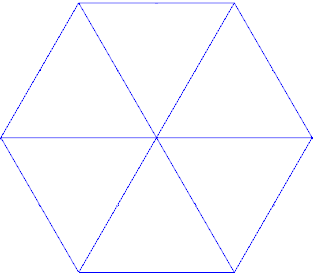
\includegraphics[width=1\linewidth]{ref4.png}}\\
\end{minipage}
\hfill
\begin{minipage}[H]{0.30\linewidth}
\center{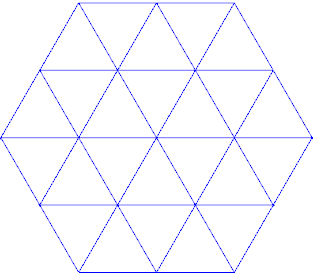
\includegraphics[width=1\linewidth]{ref0.png}}\\
\end{minipage}
\hfill
\begin{minipage}[H]{0.30\linewidth}
\center{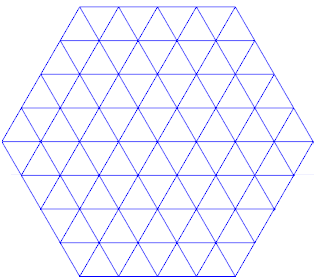
\includegraphics[width=1\linewidth]{ref1.png}}\\
\end{minipage}
\caption{Разбиение кассеты на 6, 24 и 96 конечных элементов.}
\label{ris:iaea_mesh}
\end{figure}
С целью анализа сходимости и эффективности разработанного алгоритма все тестовые расчеты были выполнены с фиксированной точностью отгонки собственного числа равной $10^{-15}$. Сравнение полученных результатов проводилось с результатами расчетов по
диффузионной мелкосеточной программе DIF3D-FD\cite{chao} (эталонное решение было
получено путем экстраполяции результатов на бесконечно малый размер
элементарной ячейки расчетной сетки).
Будем рассматривать следующие отклонения в расчетных параметрах:
\begin{itemize}\itemsep1pt \parskip0pt \parsep0pt
\item для эффективного коэффициента размножения, абсолютное отклонение от «эталонного» значения $K_{ref}$: $\Delta K = |K_{eff} - K_{ref}|$, выражается в \textit{pcm} (percent-milli, т.е. $10^{-5}$);
\item для распределения покассетных мощностей $P_i$ вычисляются относительные отклонения $\varepsilon_i$ (выраженные в \%):
\[
\varepsilon_i = \frac{P_i - P_i^{ref}}{P_i^{ref}},
\]
где $P_i^{ref}$ --- «эталонное» значение мощности в кассете $i$ ($i = 1,...,N$).
\item по отклонениям $\varepsilon_i$ рассчитываются интегральные отклонения:
\begin{itemize}\itemsep1pt \parskip0pt \parsep0pt
\item cреднеквадратическое отклонение RMS:
\[
\mathrm{RMS} = \sqrt{\frac{1}{N}\sum_{i=1}^N \varepsilon_i^2},
\]
\item среднее по модулю отклонение AVR:
\[
\mathrm{AVR} = \frac{1}{N}\sum_{i=1}^N \left\vert \varepsilon_i\right\vert,
\]
\item максимальное по модулю отклонение MAX:
\[
\mathrm{MAX} = \underset{i}{\max}\left\vert\varepsilon_i\right\vert.
\]
\end{itemize}
\end{itemize}
Определим критерии «приемлемости» результатов с точки зрения достижения достаточной для практических расчетов ВВЭР точности:
\begin{itemize}
\item отклонение $K_{eff}$ не выше 0.1\% (100 $pcm$);
\item максимальное по модулю отклонение в покассетных мощностях не выше 2\%. 
\end{itemize}
Будем считать «оптимальным» вариант, удовлетворяющий этим критериям и наиболее экономичный (по времени счета). Результаты расчетов, полученные для «оптимального» варианта будут отражены на рисунках и выделены в таблицах (серым цветом). Все вычисления проводились на компьютере со следующей конфигурацией: processor -- Intel Core i3 3.30GHz, memory -- 8Gb.
\subsection{Модифицированный тест IAEA-2D без отражателя}
\label{s-4-1}
Тестовая задача является модификацией на случай гексагональной геометрии известной тестовой задачи IAEA-2D\cite{chao}. Геометрическая модель активной зоны реактора моделируется набором кассет гексагональной формы.  Активная зона имеет 13 стрежней СУЗ (устройства систем управления и защиты реактора) и 1/12 зеркальную симметрию. Размер кассеты «под ключ»\;равен 20 см. На рисунке \ref{ris:iaea} показана геометрическая модель активной зоны, где цифрами показаны кассеты различных сортов. Диффузионные нейтронно-физические константы заданы в таблице \ref{t1}. Отражатель не моделируется, граничные условия задаются в виде логарифмической производной.   Рассматривается два варианта, отличающиеся значениями логарифмической производной на границе. \\ Результаты расчета модифицированного теста IAEA-2D без отражателя приведены в таблицах \ref{t2}, \ref{t3}. Здесь приняты следующие обозначения: $n$ --- число ячеек на кассету; $p$ --- порядок конечного элемента; $K_{eff}$ --- эффективный коэффициент размножения; $\Delta K$ --- абсолютное отклонение от «эталонного» значения; RMS --- среднеквадратичное отклонение; AVR --- среднее отклонение; MAX --- максимальное отклонение; $t$ --- время счета.\\
Распределение мощности показаны на рисунках \ref{ris:power1}, \ref{ris:power2}. Здесь для каждой кассеты сверху вних приведены: материал, «эталонное» решение, решение и относительное отклонение от «эталонного» решения.

%%Диффузионные константы для модифицированного теста IAEA-2D
\begin{table}[H]
\caption{\label{tab:canonsummary}Диффузионные константы для модифицированного теста IAEA-2D.}
\label{t1}
\begin{center}
\begin{tabular}{|c|c|c|c|c|}
\hline
Материал & 1 & 2 & 3 & 4\\
\hline 
$D_1$ & 1.500 & 1.500 & 1.500 & 1.500\\
\hline 
$D_2$ & 0.400 & 0.400 & 0.400 & 0.400\\
\hline 
$\Sigma_{a1} + \Sigma_r$ & 3.00e-2 & 3.00e-2 & 3.00e-2 & 4.00e-2\\
\hline
$\Sigma_{a2}$ & 8.00e-2 & 8.50e-2 & 1.30e-1 & 1.00e-2\\
\hline
$\Sigma_r$ & 2.00e-2 & 2.00e-2 & 2.00e-2 & 4.00e-2\\
\hline
$\Sigma_{f1}$ & 0.00 & 0.00 & 0.00 & 0.00\\
\hline
$\Sigma_{f2}$ & 5.60e-2 & 5.60e-2 & 5.60e-2 & 0.00\\
\hline
$\nu_1\Sigma_{f1}$ & 0.00 & 0.00 & 0.00 & 0.00\\
\hline
$\nu_2\Sigma_{f2}$ & 1.35e-1 & 1.35e-1 & 1.35e-1 & 0.00\\
\hline
\end{tabular}
\end{center}
\end{table}
%Геометрическая модель активной зоны модифицированного теста IAEA-2D без отражателя
\begin{figure}[H]
	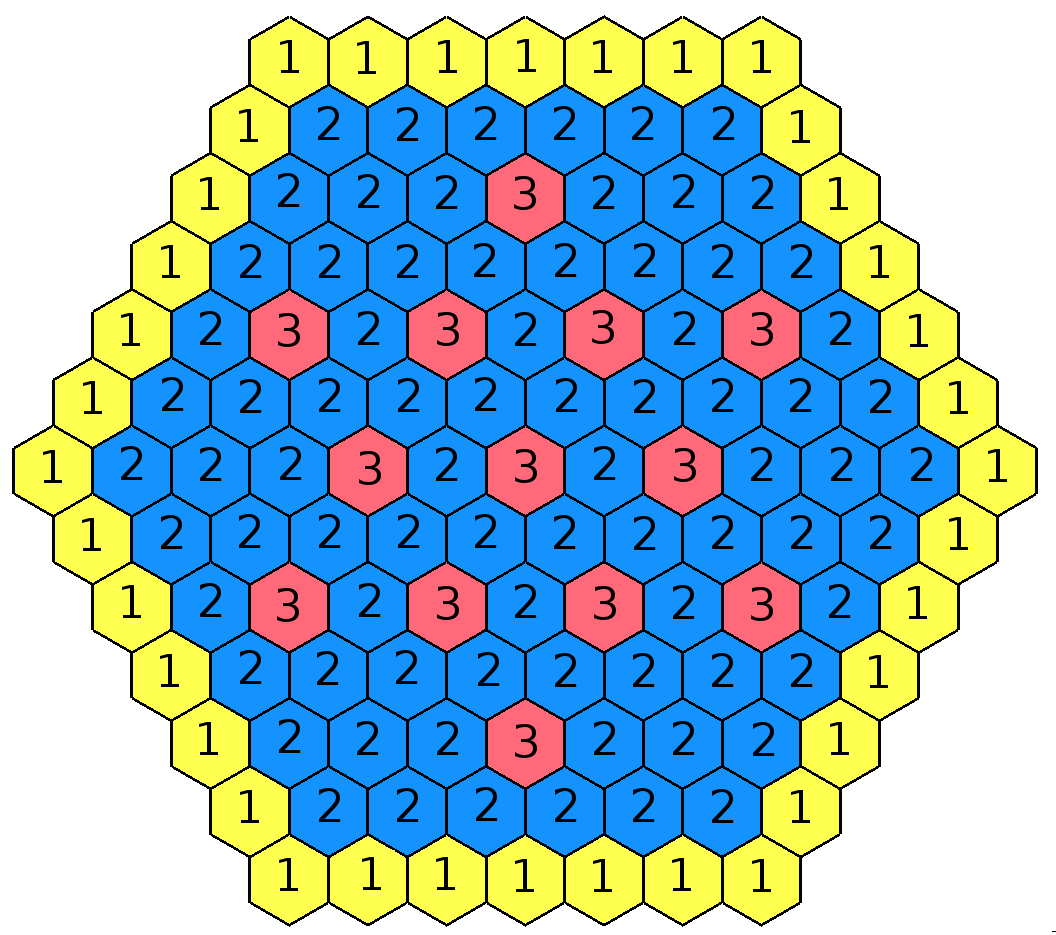
\includegraphics[width=0.85\linewidth]{iaea.png}\\
	\caption{\label{image:canonsummary}Геометрическая модель активной зоны модифицированного теста IAEA-2D без отражателя.}
	\label{ris:iaea}
\end{figure}
%Результаты расчета теста IAEA-2D без отражателя
\begin{table}[H]
\caption{\label{tab:canonsummary}Результаты расчета модифицированного теста IAEA-2D без отражателя при $\gamma = 0.5$.}
\label{t2}
\begin{center}

\rowcolors{3}{gray!50}{}
\begin{tabular}{|c|c|c|r|r|r|r|r|}
\hline
$n$ & $p$ & $K_{eff}$ & $\Delta K(\textit{pcm})$ & RMS(\%) & AVR(\%) & MAX(\%)& $t$(sec) \\
\hline
& 1 & 0.9733476 & 472.94 & 3.80 & 2.94 & 9.04 & 0.03\\
6 & 2 & 0.9775987 & 47.83 & 0.45 & 0.39 & 0.87 & 0.08\\
\hiderowcolors
& 3 & 0.9780084 & 6.86 & 0.07 & 0.06 & 0.12 & 0.19\\ \hline
\multirow{3}{*}{24} & 1 & 0.9765384 & 153.86 & 1.28 & 1.04 & 2.86 & 0.07\\
& 2 & 0.9779893 & 8.77 & 0.08 & 0.07 & 0.16 & 0.35\\
& 3 & 0.9780690 & 0.80 & 0.01 & 0.01 & 0.03 & 0.94\\ \hline
\multirow{3}{*}{96} & 1 & 0.9776501 & 42.69 & 0.36 & 0.30 & 0.79 & 0.32\\
& 2 & 0.9780655 & 1.15 & 0.02 & 0.01 & 0.03 & 2.00\\
& 3 & 0.9780757 & 0.13 & 0.01 & 0.01 & 0.02 & 5.50\\ \hline
\multirow{3}{*}{384} & 1 & 0.9779644 & 11.26 & 0.10 & 0.08 & 0.20 & 1.88\\
& 2 & 0.9780752 & 0.18 & 0.01 & 0.01 & 0.02 & 12.50\\
& 3 & 0.9780764 & 0.06 & 0.01 & 0.00 & 0.01 & 34.70\\ \hline
\multirow{3}{*}{1536}& 1 & 0.9780477 & 2.93 & 0.03 & 0.02 & 0.05 & 11.60\\
& 2 & 0.9780763 & 0.07 & 0.01 & 0.00 & 0.01 & 82.70\\
& 3 & 0.9780764 & 0.06 & 0.01 & 0.00 & 0.01 & 230.50\\ \hline
\multirow{1}{*}{Ref.}& & 0.9780770 & & & & &\\ \hline
\end{tabular}
\end{center}
\end{table}

\begin{figure}[H]
	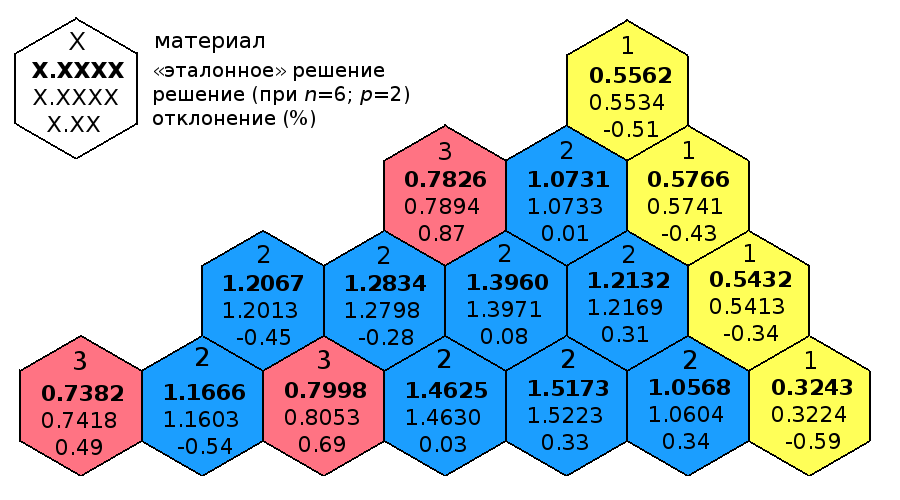
\includegraphics[width=0.85\linewidth]{power_iaea_05_6_2.png}\\
	\caption{\label{image:canonsummary}Распределение мощности для модифицированного теста IAEA-2D без отражателя при $\gamma=0.5$ .}
	\label{ris:power1}
\end{figure}

\begin{figure}[H]
	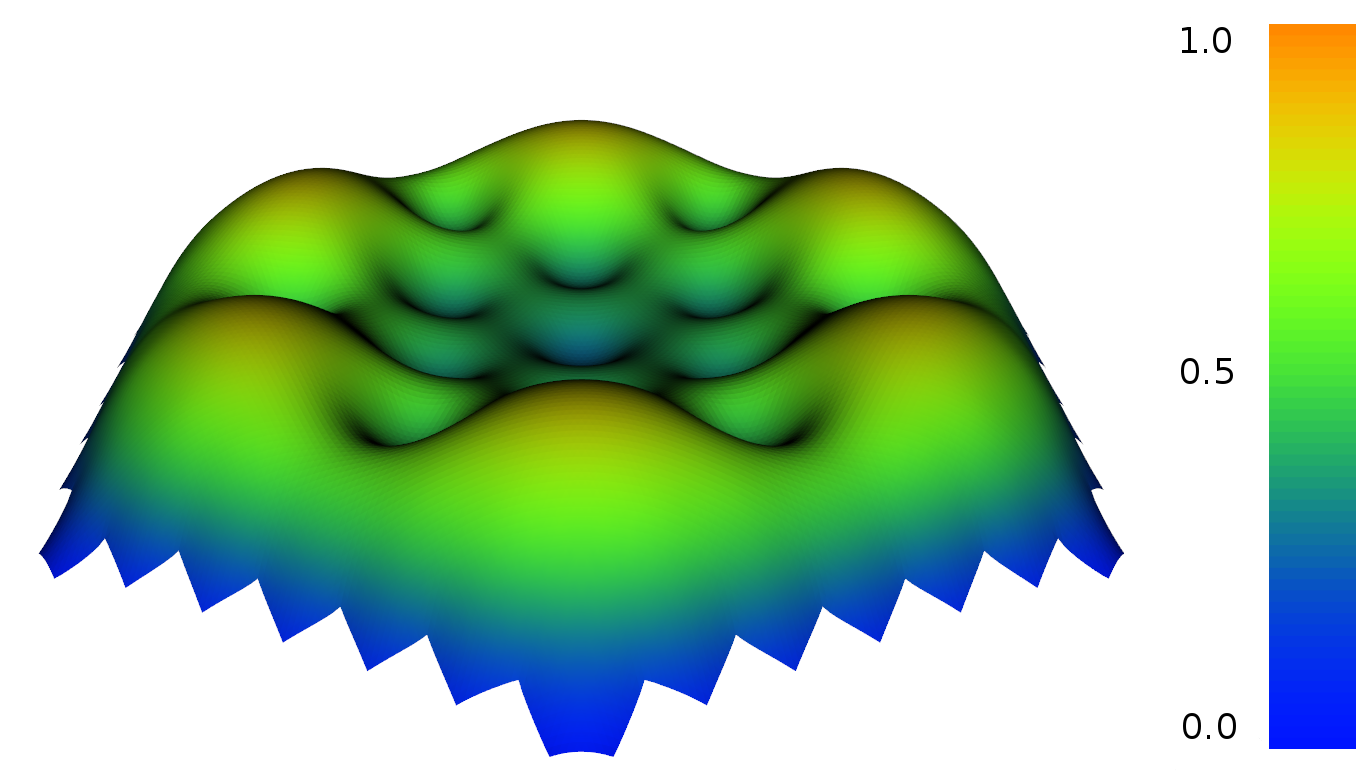
\includegraphics[width=0.85\linewidth]{power.png}\\
	\caption{\label{image:canonsummary}Плотность потока быстрых нейтронов для модифицированного теста IAEA-2D без отражателя при $\gamma=0.5, n=1536, p=1$.}
	\label{ris:power}
\end{figure}

\begin{table}[H]
\caption{\label{tab:canonsummary}Результаты расчета модифицированного теста IAEA-2D без отражателя при $\gamma = 0.125$.}
\label{t3}
\begin{center}
\rowcolors{3}{gray!50}{}
\begin{tabular}{|c|c|c|r|r|r|r|r|}
\hline
$n$ & $p$ & $K_{eff}$ & $\Delta K(\textit{pcm})$ & RMS(\%) & AVR(\%) & MAX(\%) & $t$(sec) \\
\hline
& 1 & 0.9877260 & 365.20 & 3.65 & 2.66 & 8.40 & 0.03 \\
6 & 2 & 0.9910086 & 36.94 & 0.39 & 0.28 & 0.80 & 0.08\\
\hiderowcolors
& 3 & 0.9913262 & 5.18 & 0.06 & 0.04 & 0.12 & 0.20\\ \hline
\multirow{3}{*}{24} & 1 & 0.9901896 & 118.84 & 1.21 & 0.88 & 2.65 & 0.08\\
& 2 & 0.9913114 & 6.66 & 0.07 & 0.05 & 0.15 & 0.36\\
& 3 & 0.9913743 & 0.37 & 0.01 & 0.01 & 0.02 & 0.99\\ \hline
\multirow{3}{*}{96} & 1 & 0.9910477 & 33.03 & 0.34 & 0.25 & 0.74 & 0.34\\
& 2 & 0.9913713 & 0.67 & 0.01 & 0.01 & 0.02 & 2.10\\
& 3 & 0.9913789 & 0.09 & 0.00 & 0.00 & 0.01 & 5.70\\ \hline
\multirow{3}{*}{384} & 1 & 0.9912924 & 8.56 & 0.09 & 0.07 & 0.20 & 1.96\\
& 2 & 0.9913785 & 0.05 & 0.01 & 0.00 & 0.01 & 12.80\\
& 3 & 0.9913792 & 0.12 & 0.00 & 0.00 & 0.01 & 35.00\\ \hline
\multirow{3}{*}{1536}& 1 & 0.9913571 & 2.09 & 0.02 & 0.02 & 0.06 & 12.00\\
& 2 & 0.9913792 & 0.12 & 0.00 & 0.00 & 0.01 & 83.00\\
& 3 & 0.9913793 & 0.13 & 0.00 & 0.00 & 0.01 & 231.50\\ \hline
\multirow{1}{*}{Ref.}& & 0.9913780 & & & & &\\ \hline
\end{tabular}
\end{center}
\end{table}

\begin{figure}[H]
	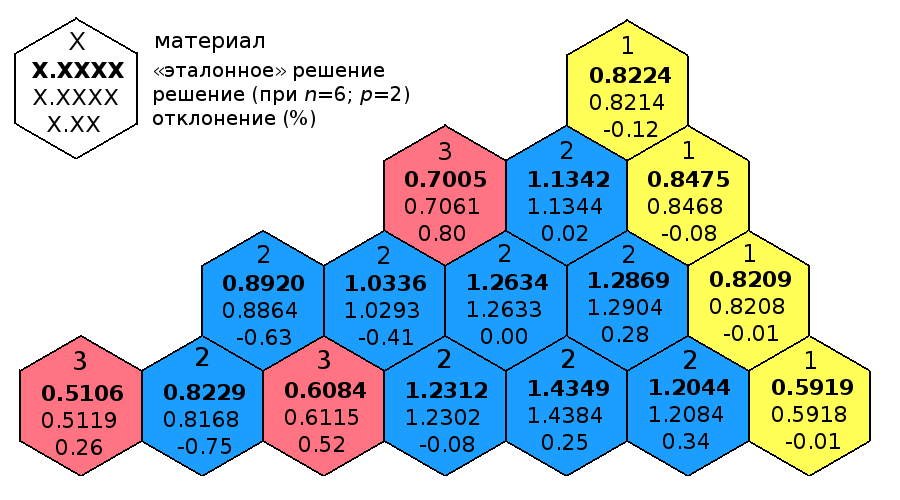
\includegraphics[width=0.85\linewidth]{power_iaea_0125_6_2.png}\\
	\caption{\label{image:canonsummary}Распределение мощности для модифицированного теста IAEA-2D без отражателя при $\gamma=0.125$.}
	\label{ris:power2}
\end{figure}


\subsection{Модифицированный тест IAEA-2D с отражателем}
\label{s-4-2}
Тестовая задача аналогична предыдущей, за исключением того, что был добавлен внешний ряд отражателя (материал 4). Диффузионные нейтронно-физические константы заданы в таблице \ref{t1}. Граничные условия задаются в виде логарифмической производной. Так же рассматривается два варианта, отличающиеся значениями логарифмической производной на границе. Результаты расчета модифицированного теста IAEA-2D с отражателем приведены в таблицах \ref{t4}, \ref{t5} и на рисунках \ref{ris:power3}, \ref{ris:power4}.
\begin{table}[H]
\caption{\label{tab:canonsummary}Результаты расчета модифицированного теста IAEA-2D с отражателем при $\gamma = 0.5$.}
\label{t4}
\begin{center}
\rowcolors{4}{}{gray!50}
\begin{tabular}{|c|c|c|r|r|r|r|r|}
\hline
$n$ & $p$ & $K_{eff}$ & $\Delta K(\textit{pcm})$ & RMS(\%) & AVR(\%) & MAX(\%)& $t$(sec) \\
\hline
\multirow{3}{*}{6} & 1 & 1.0104126 & 490.56 & 13.29 & 11.13 & 23.73 & 0.03\\
& 2 & 1.0062265 & 71.95 & 1.88 & 1.59 & 3.40 & 0.11\\
& 3 & 1.0055754 & 6.84 & 0.22 & 0.18 & 0.41 & 0.27\\ \hline
\hiderowcolors
\multirow{3}{*}{24} & 1 & 1.0069873 & 148.03 & 4.54 & 3.77 & 8.45 & 0.10\\
& 2 & 1.0056090 & 10.20 & 0.30 & 0.25 & 0.57 & 0.54\\
& 3 & 1.0055135 & 0.65 & 0.02 & 0.02 & 0.04 & 1.46\\ \hline
\multirow{3}{*}{96} & 1 & 1.0059079 & 40.90 & 1.28 & 1.06 & 2.41 & 0.50\\
& 2 & 1.0055186 & 1.16 & 0.04 & 0.03 & 0.07 & 3.00\\
& 3 & 1.0055097 & 0.27 & 0.01 & 0.01 & 0.02 & 8.30\\ \hline
\multirow{3}{*}{384} & 1 & 1.0056119 & 10.49 & 0.34 & 0.28 & 0.64 & 2.95\\
& 2 & 1.0055102 & 0.32 & 0.01 & 0.01 & 0.02 & 18.70\\
& 3 & 1.0055096 & 0.26 & 0.01 & 0.01 & 0.02 & 52.00\\ \hline
\multirow{3}{*}{1536}& 1 & 1.0055354 & 2.84 & 0.09 & 0.08 & 0.17 & 18.65\\
& 2 & 1.0055096 & 0.26 & 0.01 & 0.01 & 0.02 & 132.30\\
& 3 & 1.0055096 & 0.26 & 0.01 & 0.01 & 0.02 & 370.50\\ \hline
\multirow{1}{*}{Ref.}& & 1.0055070 & & & & &\\ \hline
\end{tabular}
\end{center}
\end{table}

\begin{figure}[H]
	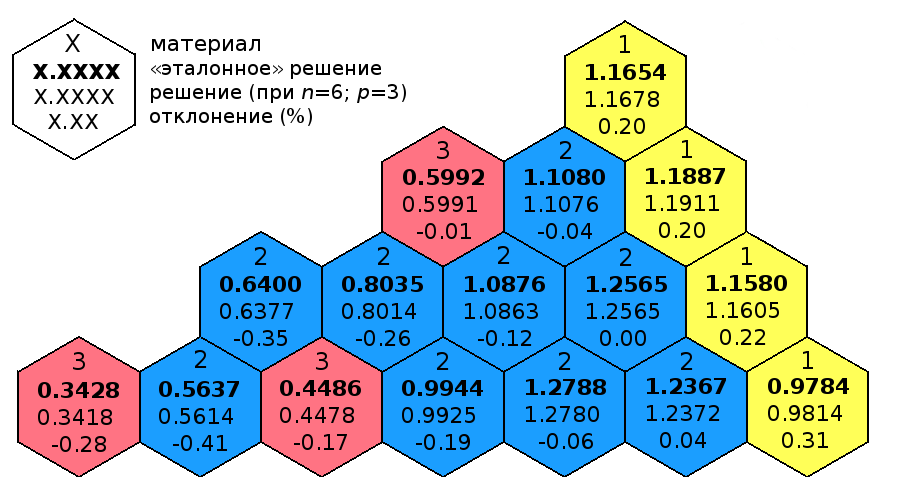
\includegraphics[width=0.85\linewidth]{power_iaea_ref_05_6_3.png}\\
	\caption{\label{image:canonsummary}Распределение мощности для модифицированного теста IAEA-2D с отражателем при $\gamma=0.5$.}
	\label{ris:power3}
\end{figure}

\begin{table}[H]
\caption{\label{tab:canonsummary}Результаты расчета модифицированного теста IAEA-2D с отражателем при $\gamma = 0.125$.}
\label{t5}
\begin{center}
\rowcolors{4}{}{gray!50}
\begin{tabular}{|c|c|c|r|r|r|r|r|}
\hline
$n$ & $p$ & $K_{eff}$ & $\Delta K(\textit{pcm})$ & RMS(\%) & AVR(\%) & MAX(\%)& $t$(sec) \\
\hline
\multirow{3}{*}{6} & 1 & 1.0120630 & 543.3 & 13.72 & 11.55 & 24.47 & 0.03\\
& 2 & 1.0074831 & 85.31 & 2.00 & 1.69 & 3.60 & 0.11\\
& 3 & 1.0067469 & 11.69 & 0.23 & 0.19 & 0.44 & 0.27\\ \hline
\hiderowcolors
\multirow{3}{*}{24} & 1 & 1.0083333 & 170.33 & 4.74 & 3.95 & 8.80 & 0.10\\
& 2 & 1.0067838 & 15.38 & 0.32 & 0.27 & 0.60 & 0.54\\
& 3 & 1.0066733 & 4.33 & 0.02 & 0.02 & 0.04 & 1.46\\ \hline
\multirow{3}{*}{96} & 1 & 1.0071200 & 49.00 & 1.34 & 1.11 & 2.52 & 0.50\\
& 2 & 1.0066790 & 4.9 & 0.04 & 0.03 & 0.07 & 3.00\\
& 3 & 1.0066682 & 3.82 & 0.01 & 0.01 & 0.01 & 8.30\\ \hline
\multirow{3}{*}{384} & 1 & 1.0067847 & 15.47 & 0.35 & 0.29 & 0.67 & 2.95\\
& 2 & 1.0066688 & 3.88 & 0.01 & 0.01 & 0.02 & 18.70\\
& 3 & 1.0066680 & 3.8 & 0.01 & 0.01 & 0.01 & 52.00\\ \hline
\multirow{3}{*}{1536}& 1 & 1.0066975 & 6.75 & 0.09 & 0.08 & 0.18 & 18.65\\
& 2 & 1.0066680 & 3.8 & 0.01 & 0.01 & 0.01 & 132.30\\
& 3 & 1.0066680 & 3.8 & 0.01 & 0.01 & 0.01 & 370.50\\ \hline
\multirow{1}{*}{Ref.}& & 1.0066300 & & & & &\\ \hline
\end{tabular}
\end{center}
\end{table}

\begin{figure}[H]
	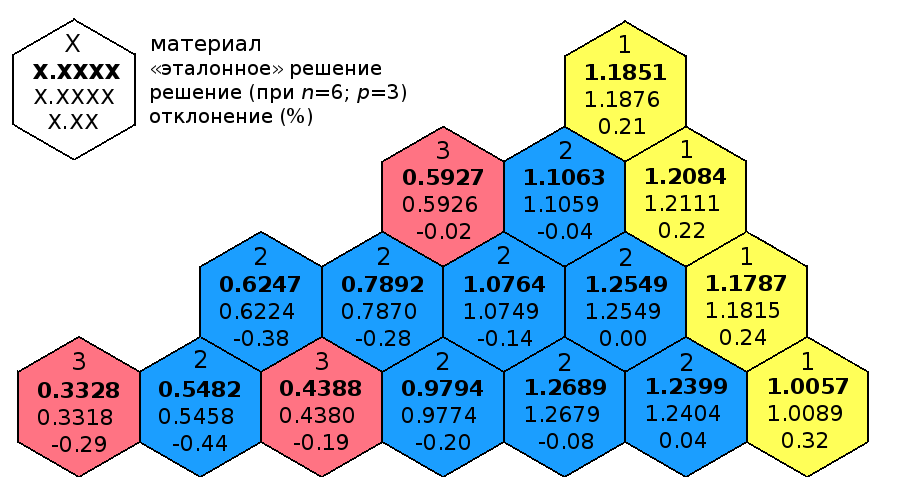
\includegraphics[width=0.85\linewidth]{power_iaea_ref_0125_6_3.png}\\
	\caption{\label{image:canonsummary}Распределение мощности для модифицированного теста IAEA-2D с отражателем при $\gamma=0.125$.}
	\label{ris:power4}
\end{figure}

\subsection{Двухмерная модель ВВЭР-1000 без отражателя}
\label{s-4-3}
Геометрическая модель активной зоны ВВЭР-1000 моделируется набором кассет гексагональной формы. На рисунке \ref{ris:vver1000} показана геометрическая модель активной зоны ВВЭР-1000, где цифрами показаны кассеты различных сортов.
Размер кассеты «под ключ»\;равен 23.6 см. Активная зона имеет 25 стержней СУЗ и 1/6 зеркальную симметрию. Диффузионные нейтронно-физические константы заданы  в таблице \ref{t6}. На внешней границе реактора задается условие границы с вакуумом (логарифмическая производная  $\gamma = 0.5$) и более реалистичные условия (логарифмическая производная  $\gamma = 0.125$). Результаты расчета двухмерного теста ВВЭР-1000 без отражателя приведены в таблицах \ref{t7}, \ref{t8} и на рисунках \ref{ris:power5}, \ref{ris:power6}.
%Геометрическая модель активной зоны двухмерной модели ВВЭР-1000 без отражателя
\begin{figure}[H]
	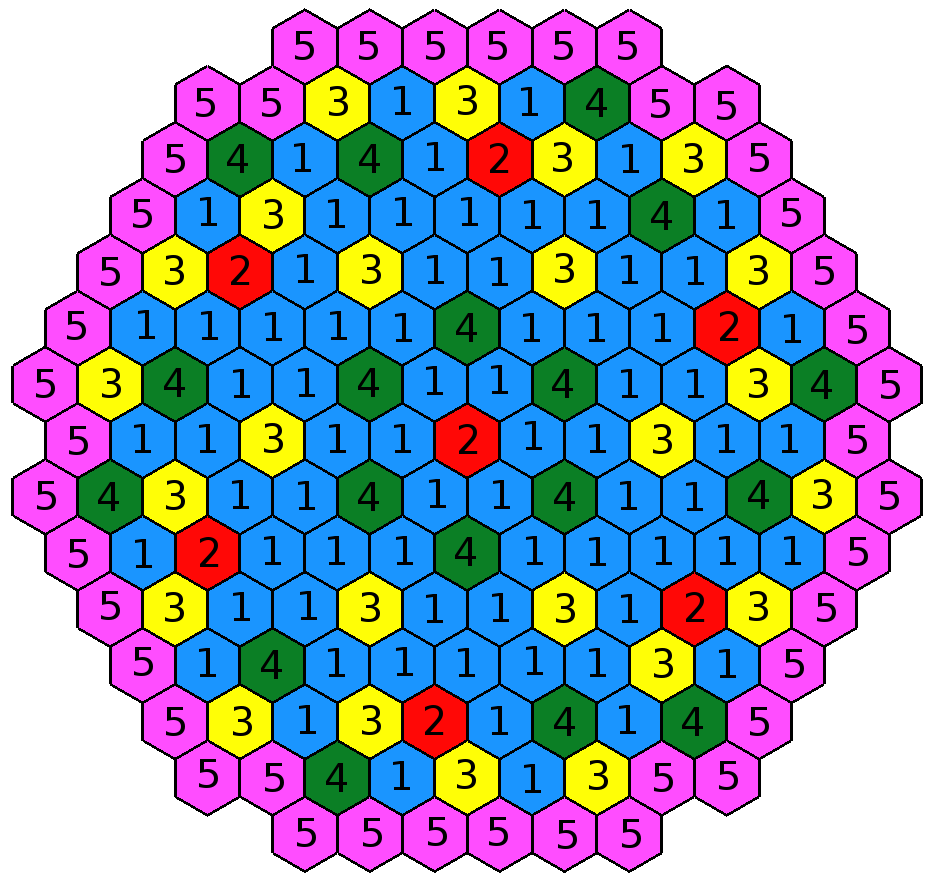
\includegraphics[width=0.75\linewidth]{vver.png}\\
	\caption{\label{image:canonsummary}Геометрическая модель активной зоны двухмерной модели ВВЭР-1000 без отражателя.}
	\label{ris:vver1000}
\end{figure}

%Диффузионные константы для ВВЭР-1000
\begin{table}[H]
\caption{\label{tab:canonsummary}Диффузионные константы для ВВЭР-1000.}
\label{t6}
\begin{center}
\begin{tabular}{|c|c|c|c|c|c|}
\hline
Материал & 1 & 2 & 3 & 4 & 5\\
\hline 
$D_1$ & 1.3832 & 1.38299 & 1.39522 & 1.39446 & 1.39506\\
\hline 
$D_2$ & 0.386277 & 0.389403 & 0.386225 & 0.387723 & 0.384492\\
\hline 
$\Sigma_{a1} + \Sigma_r$ & 2.48836e-2 & 2.62865e-2 & 2.45662e-2 & 2.60117e-2 & 2.46141e-2\\
\hline
$\Sigma_{a2}$ & 6.73049e-2 & 8.10328e-2 & 8.44801e-1 & 9.89671e-2 & 8.93878e-2\\
\hline
$\Sigma_r$ & 1.64977e-2 & 1.47315e-2 & 1.56219e-2 & 1.40185e-2 & 1.54981e-2\\
\hline
$\Sigma_{f1}$ & 1.86139е-3 & 1.81560е-3 & 2.36371е-3 & 2.31026е-3 & 2.50773е-3\\
\hline
$\Sigma_{f2}$ & 3.48111е-2 & 3.50622е-2 & 4.91322е-2 & 4.95721е-2 & 5.31856е-2\\
\hline
$\nu_1\Sigma_{f1}$ & 4.81619e-3 & 4.66953e-3 & 6.04889e-3 & 5.91507e-3 & 6.40256e-3\\
\hline
$\nu_2\Sigma_{f2}$ & 8.46154e-2 & 8.52264e-2 & 1.19428e-1 & 1.20497e-1 & 1.29281e-1\\
\hline
\end{tabular}
\end{center}
\end{table}

\begin{table}[H]
\caption{\label{tab:canonsummary}Результаты расчета двухмерного теста ВВЭР-1000 без отражателя при $\gamma = 0.5$.}
\label{t7}
\begin{center}
\rowcolors{3}{gray!50}{}
\begin{tabular}{|c|c|c|r|r|r|r|r|}
\hline
$n$ & $p$ & $K_{eff}$ & $\Delta K(\textit{pcm})$ & RMS(\%) & AVR(\%) & MAX(\%)& $t$(sec) \\
\hline
& 1 & 1.0048221 & 166.29 & 5.71 & 4.57 & 12.07 & 0.03\\
6 & 2 & 1.0063892 & 9.58 & 0.66 & 0.52 & 1.41 & 0.12\\
\hiderowcolors
& 3 & 1.0064425 & 4.25 & 0.14 & 0.11 & 0.28 & 0.30\\ \hline
\multirow{3}{*}{24} & 1 & 1.0059909 & 49.41& 1.94 & 1.55 & 4.20 & 0.12\\
& 2 & 1.0064407 & 4.43 & 0.16 & 0.13 & 0.32 & 0.59\\
& 3 & 1.0064454 & 3.96 & 0.08 & 0.07 & 0.15 & 1.61\\ \hline
\multirow{3}{*}{96} & 1 & 1.0063266 & 15.84 & 0.58 & 0.47 & 1.25 & 0.54\\
& 2 & 1.0064455 & 3.95 & 0.08 & 0.07 & 0.15 & 3.37\\
& 3 & 1.0064466 & 3.84 & 0.07 & 0.06 & 0.14 & 8.96\\ \hline
\multirow{3}{*}{384} & 1 & 1.0064156 & 6.94 & 0.19 & 0.16 & 0.37 & 3.15\\
& 2 & 1.0064466 & 3.84 & 0.07 & 0.06 & 0.14 & 19.77\\
& 3 & 1.0064469 & 3.81 & 0.07 & 0.06 & 0.14 & 55.00\\ \hline
\multirow{3}{*}{1536}& 1 & 1.0064389 & 4.61 & 0.10 & 0.08 & 0.17 & 18.00\\
& 2 & 1.0064469 & 3.81 & 0.07 & 0.06 & 0.14 & 129.70\\
& 3 & 1.0064469 & 3.81 & 0.07 & 0.06 & 0.14 & 366.50\\ \hline
\multirow{1}{*}{Ref.}& & 1.0064850 & & & & &\\ \hline
\end{tabular}
\end{center}
\end{table}

\begin{figure}[H]
	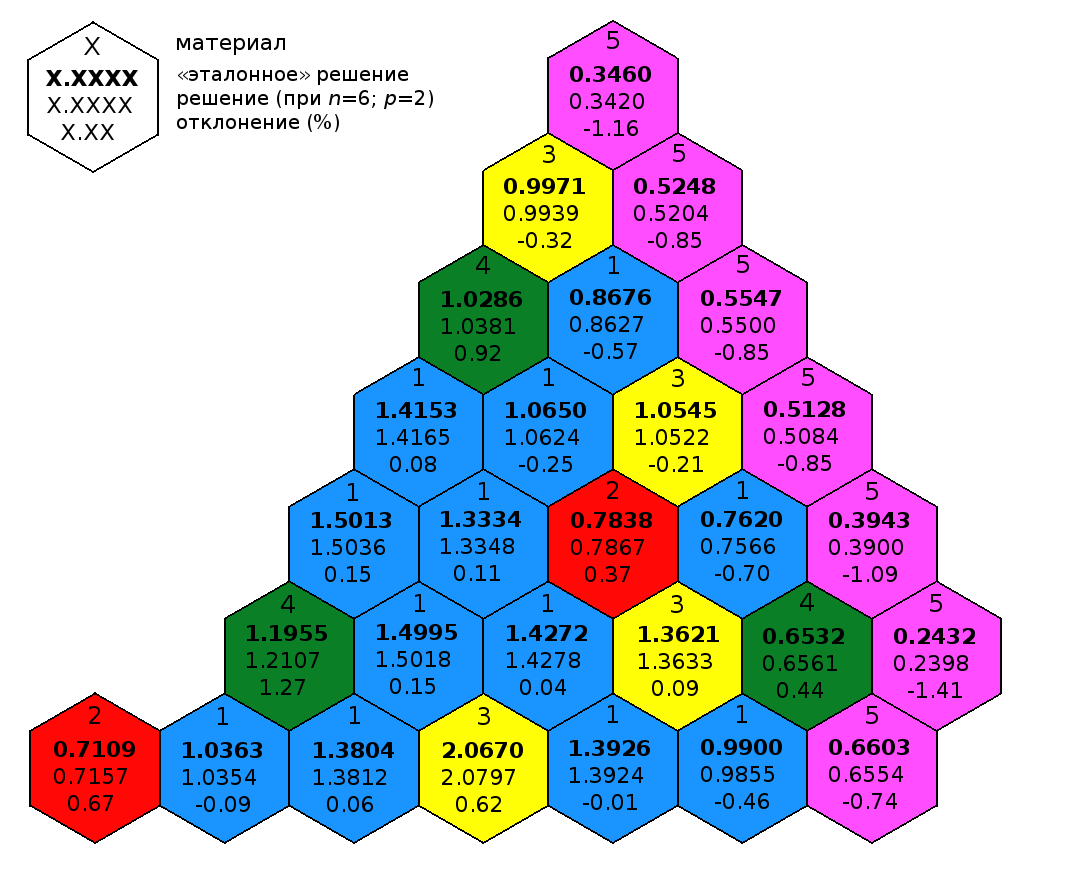
\includegraphics[width=0.75\linewidth]{power_vver_05_6_2.png}\\
	\caption{\label{image:canonsummary}Распределение мощности для модели ВВЭР-1000 без отражателя при $\gamma=0.5$.}
	\label{ris:power5}
\end{figure}

\begin{figure}[H]
	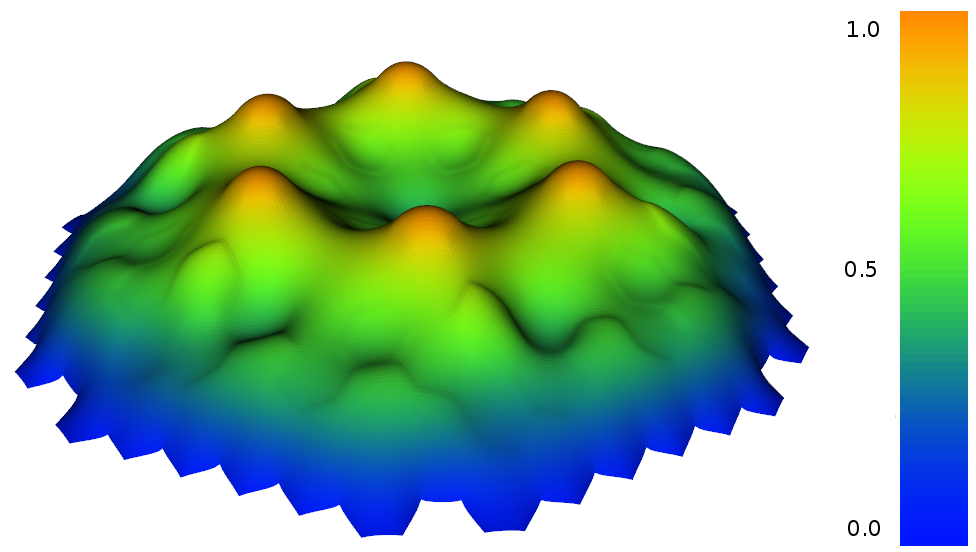
\includegraphics[width=0.85\linewidth]{power7.png}\\
	\caption{\label{image:canonsummary}Плотность потока быстрых нейтронов для модели ВВЭР-1000 без отражателя при $\gamma=0.5, n=1536, p=1$.}
	\label{ris:power7}
\end{figure}

\begin{table}[H]
\small
\caption{\label{tab:canonsummary}Результаты расчета двухмерного теста ВВЭР-1000 без отражателя при $\gamma = 0.125$.}
\label{t8}
\begin{center}
\rowcolors{3}{gray!50}{}
\begin{tabular}{|c|c|c|r|r|r|r|r|}
\hline
$n$ & $p$ & $K_{eff}$ & $\Delta K(\textit{pcm})$ & RMS(\%) & AVR(\%) & MAX(\%)& $t$(sec) \\
\hline
& 1 & 1.0125412 & 186.58 & 4.74 & 3.88 & 11.75 & 0.04\\
6 & 2 & 1.0142977 & 10.93 & 0.49 & 0.38 & 1.31 & 0.13\\
\hiderowcolors
& 3 & 1.0143626 & 4.44 & 0.11 & 0.09 & 0.30 & 0.32\\ \hline
\multirow{3}{*}{24} & 1 & 1.0138537 & 55.33 & 1.54 & 1.26 & 3.83 & 0.12\\
& 2 & 1.0143603 & 4.67 & 0.12 & 0.10 & 0.34 & 0.62\\
& 3 & 1.0143685 & 3.85 & 0.07 & 0.06 & 0.13 & 1.69\\ \hline
\multirow{3}{*}{96} & 1 & 1.0142317 & 17.53 & 0.46 & 0.38 & 1.15 & 0.57\\
& 2 & 1.0143684 & 3.86 & 0.07 & 0.06 & 0.14 & 3.51\\
& 3 & 1.0143698 & 3.72 & 0.06 & 0.05 & 0.12 & 9.32\\ \hline
\multirow{3}{*}{384} & 1 & 1.0143340 & 7.30 & 0.15 & 0.13 & 0.39 & 3.03\\
& 2 & 1.0143698 & 3.72 & 0.06 & 0.05 & 0.12 & 19.62\\
& 3 & 1.0143701 & 3.69 & 0.06 & 0.05 & 0.12 & 54.00\\ \hline
\multirow{3}{*}{1536}& 1 & 1.0143608 & 4.62 & 0.08 & 0.07 & 0.18 & 18.6\\
& 2 & 1.0143701 & 3.69 & 0.06 & 0.05 & 0.12 & 134.00\\
& 3 & 1.0143701 & 3.69 & 0.06 & 0.05 & 0.12 & 378.70\\ \hline
\multirow{1}{*}{Ref.}& & 1.0144070 & & & & &\\ \hline
\end{tabular}
\end{center}
\end{table}

\begin{figure}[H]
	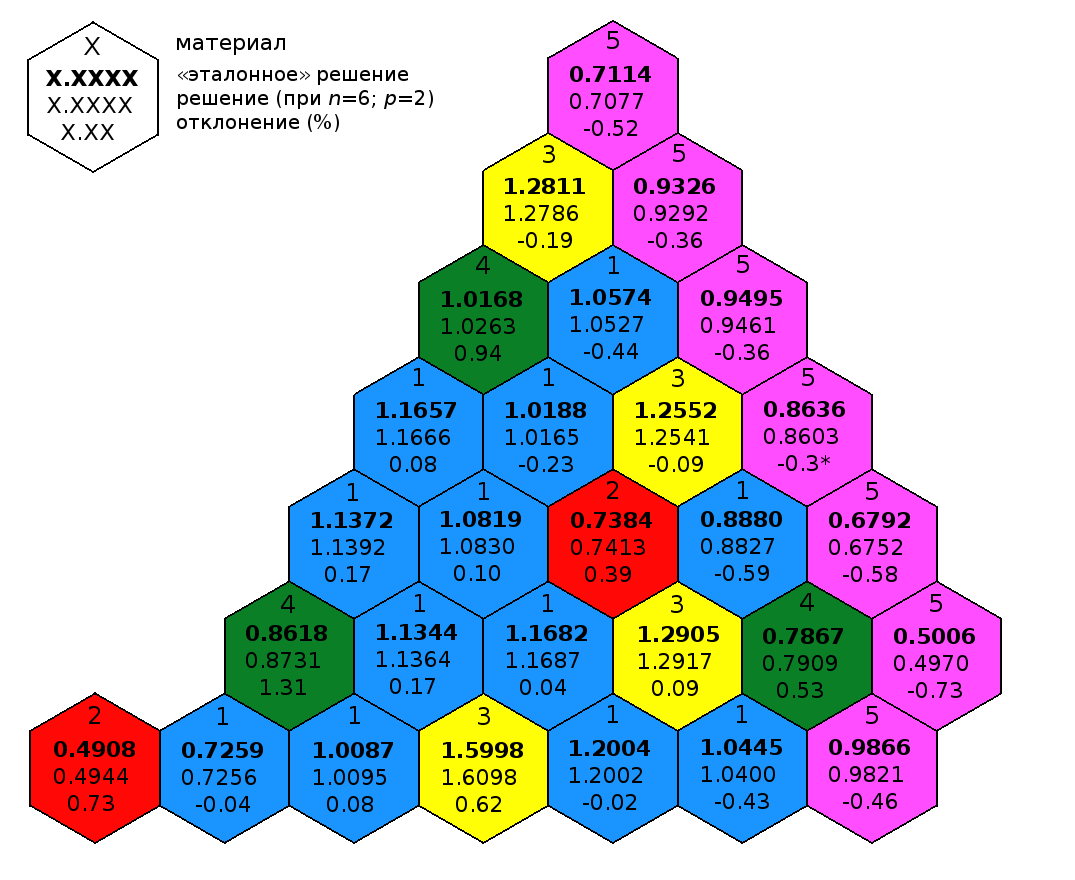
\includegraphics[width=0.70\linewidth]{power_vver_0125_6_2.png}\\
	\caption{\label{image:canonsummary}Распределение мощности для модели ВВЭР-1000 без отражателя при $\gamma=0.125$.}
	\label{ris:power6}
\end{figure}

\subsection{Анализ результатов расчетов}
\label{s-4-4}
Для иллюстрации результатов расчета тестовых задач по разработанному алгоритму рассмотрим несколько графиков для первой тестовой задачи. На рисунках 12-14 приведены кривые отклонения $\Delta K$, максимального отклонения мощности MAX и времени счета задачи $t$ в зависимости от числа конечных элементов на кассету $n$ и порядка конечных элементов $p$. 

\begin{figure}[H]
	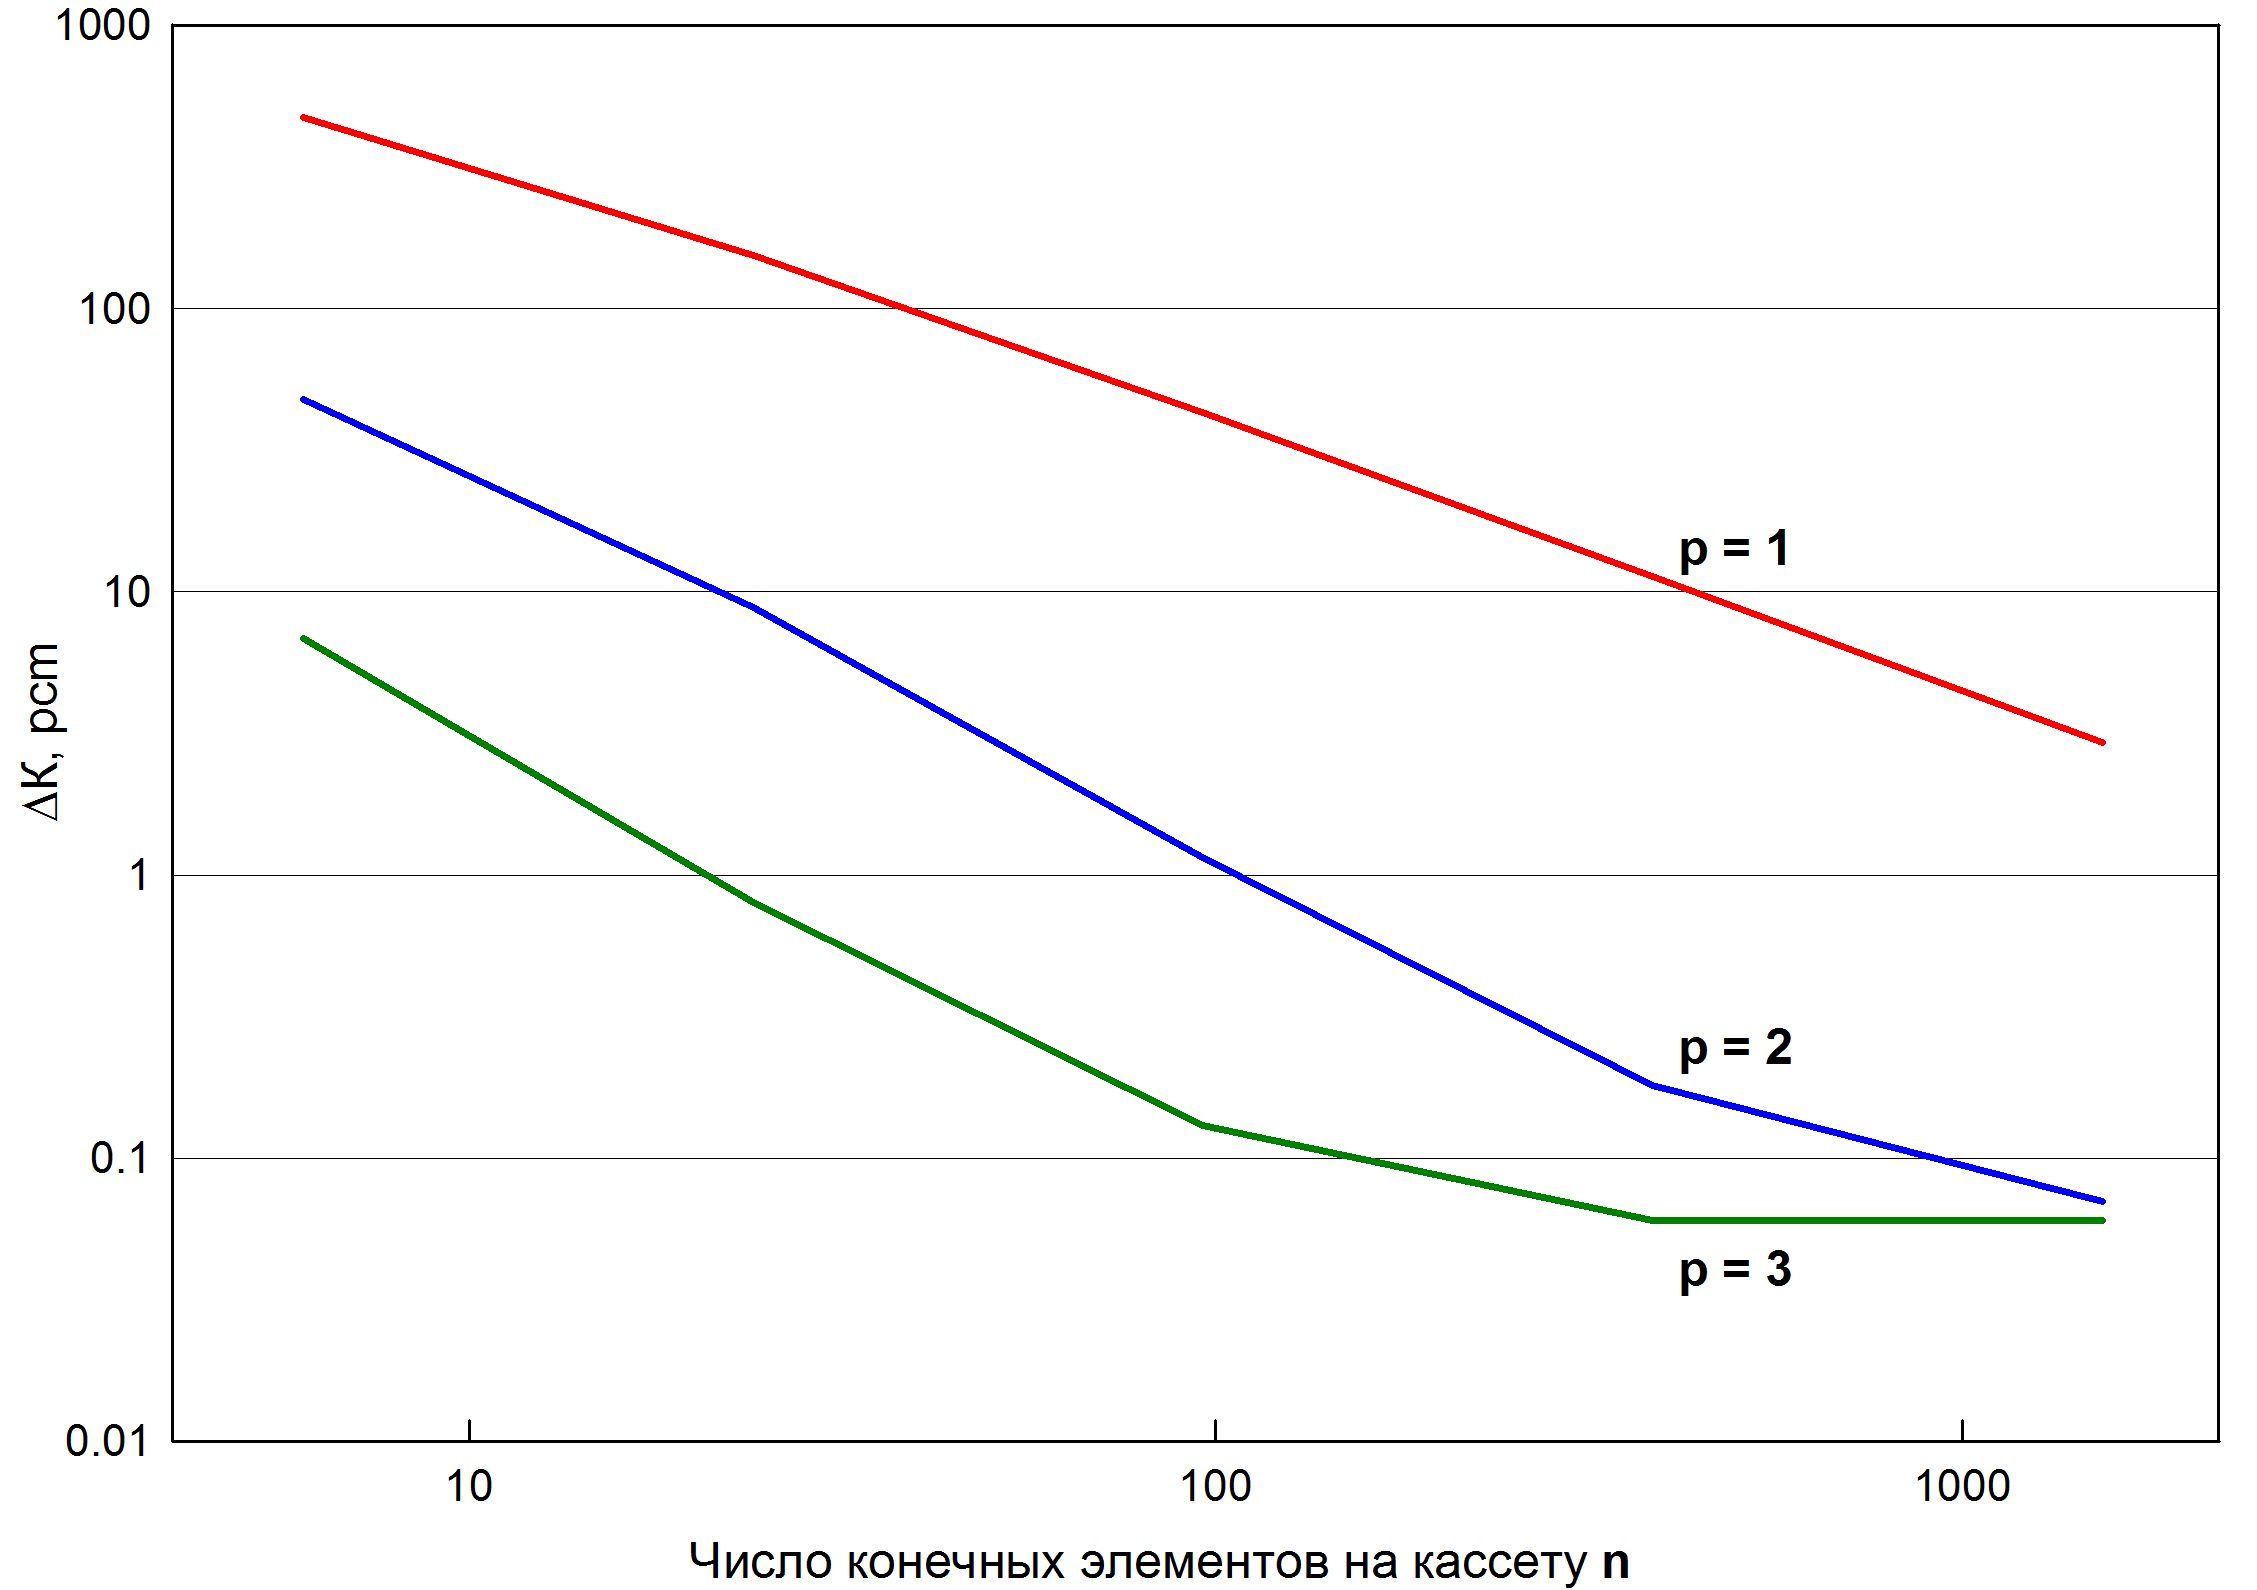
\includegraphics[width=1\linewidth]{KeffErr.png}\\
	\caption{\label{image:canonsummary}Отклонение коэффициента размножения, $\Delta K$.}
	\label{ris:graph2}
\end{figure}
$\phantom{123}$\\\\
\begin{figure}[H]
	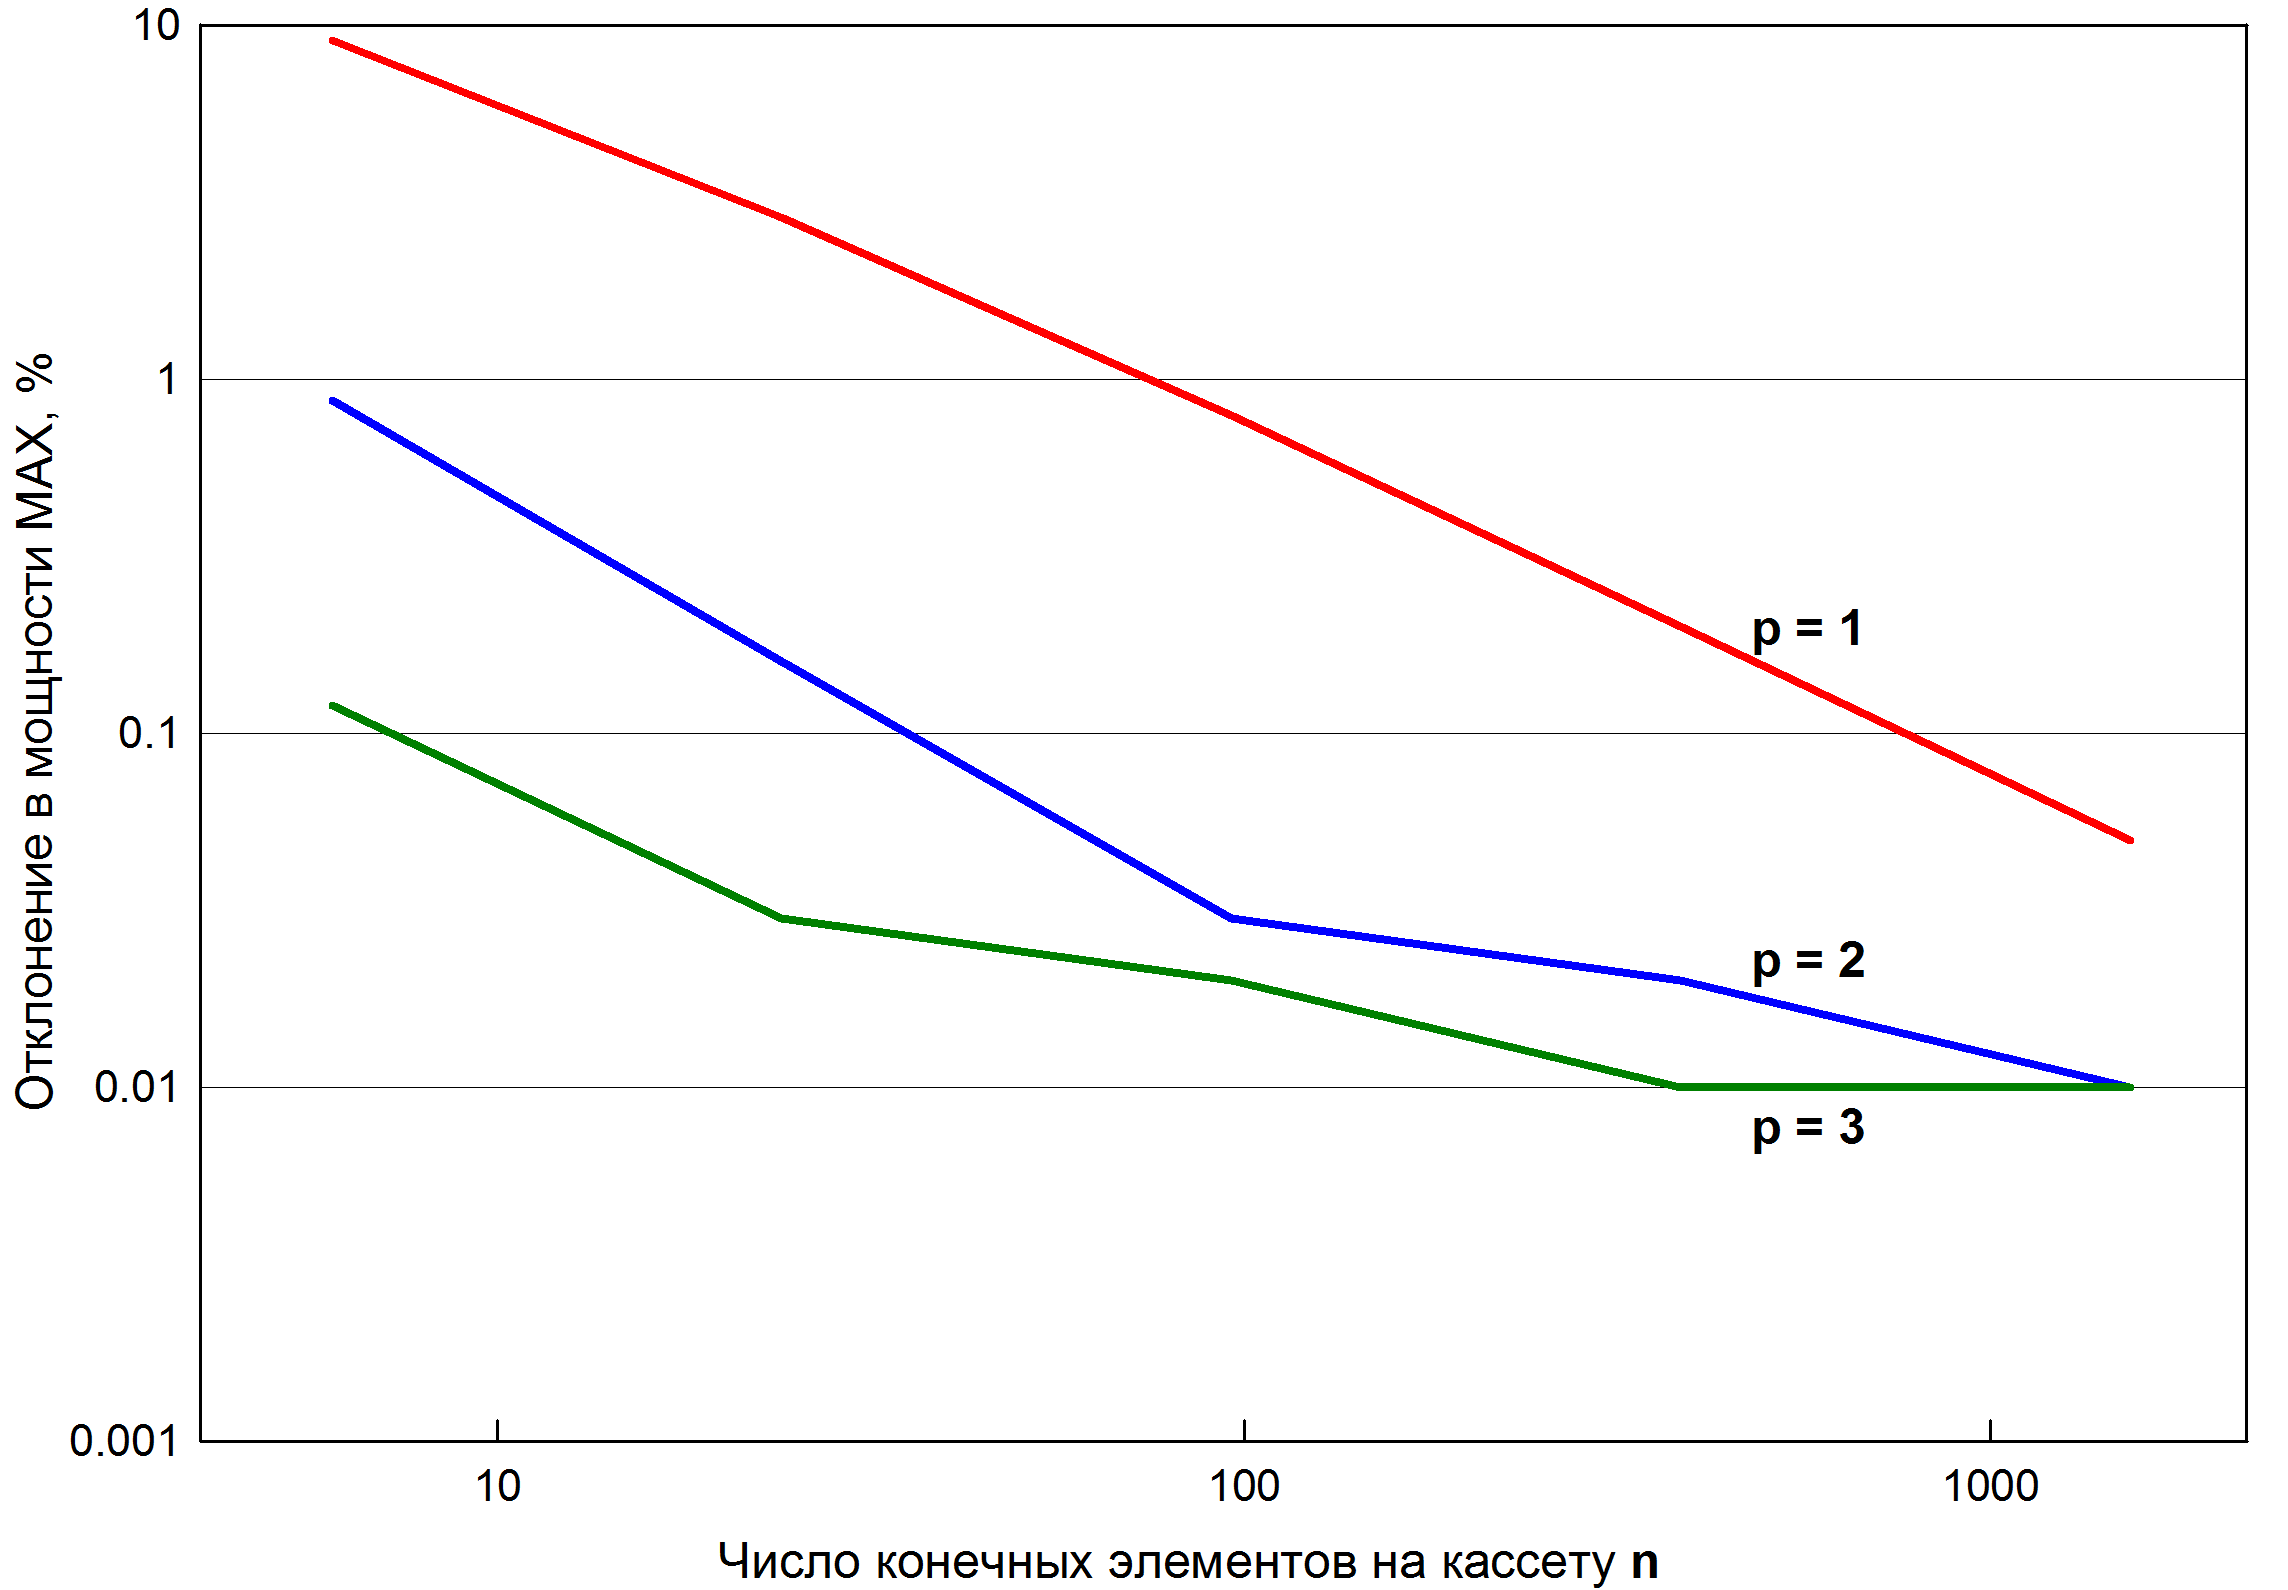
\includegraphics[width=0.9\linewidth]{MaxErr.png}\\
	\caption{\label{image:canonsummary}Максимальное отклонение мощности, MAX.}
	\label{ris:graph3}
\end{figure}

\begin{figure}[H]
	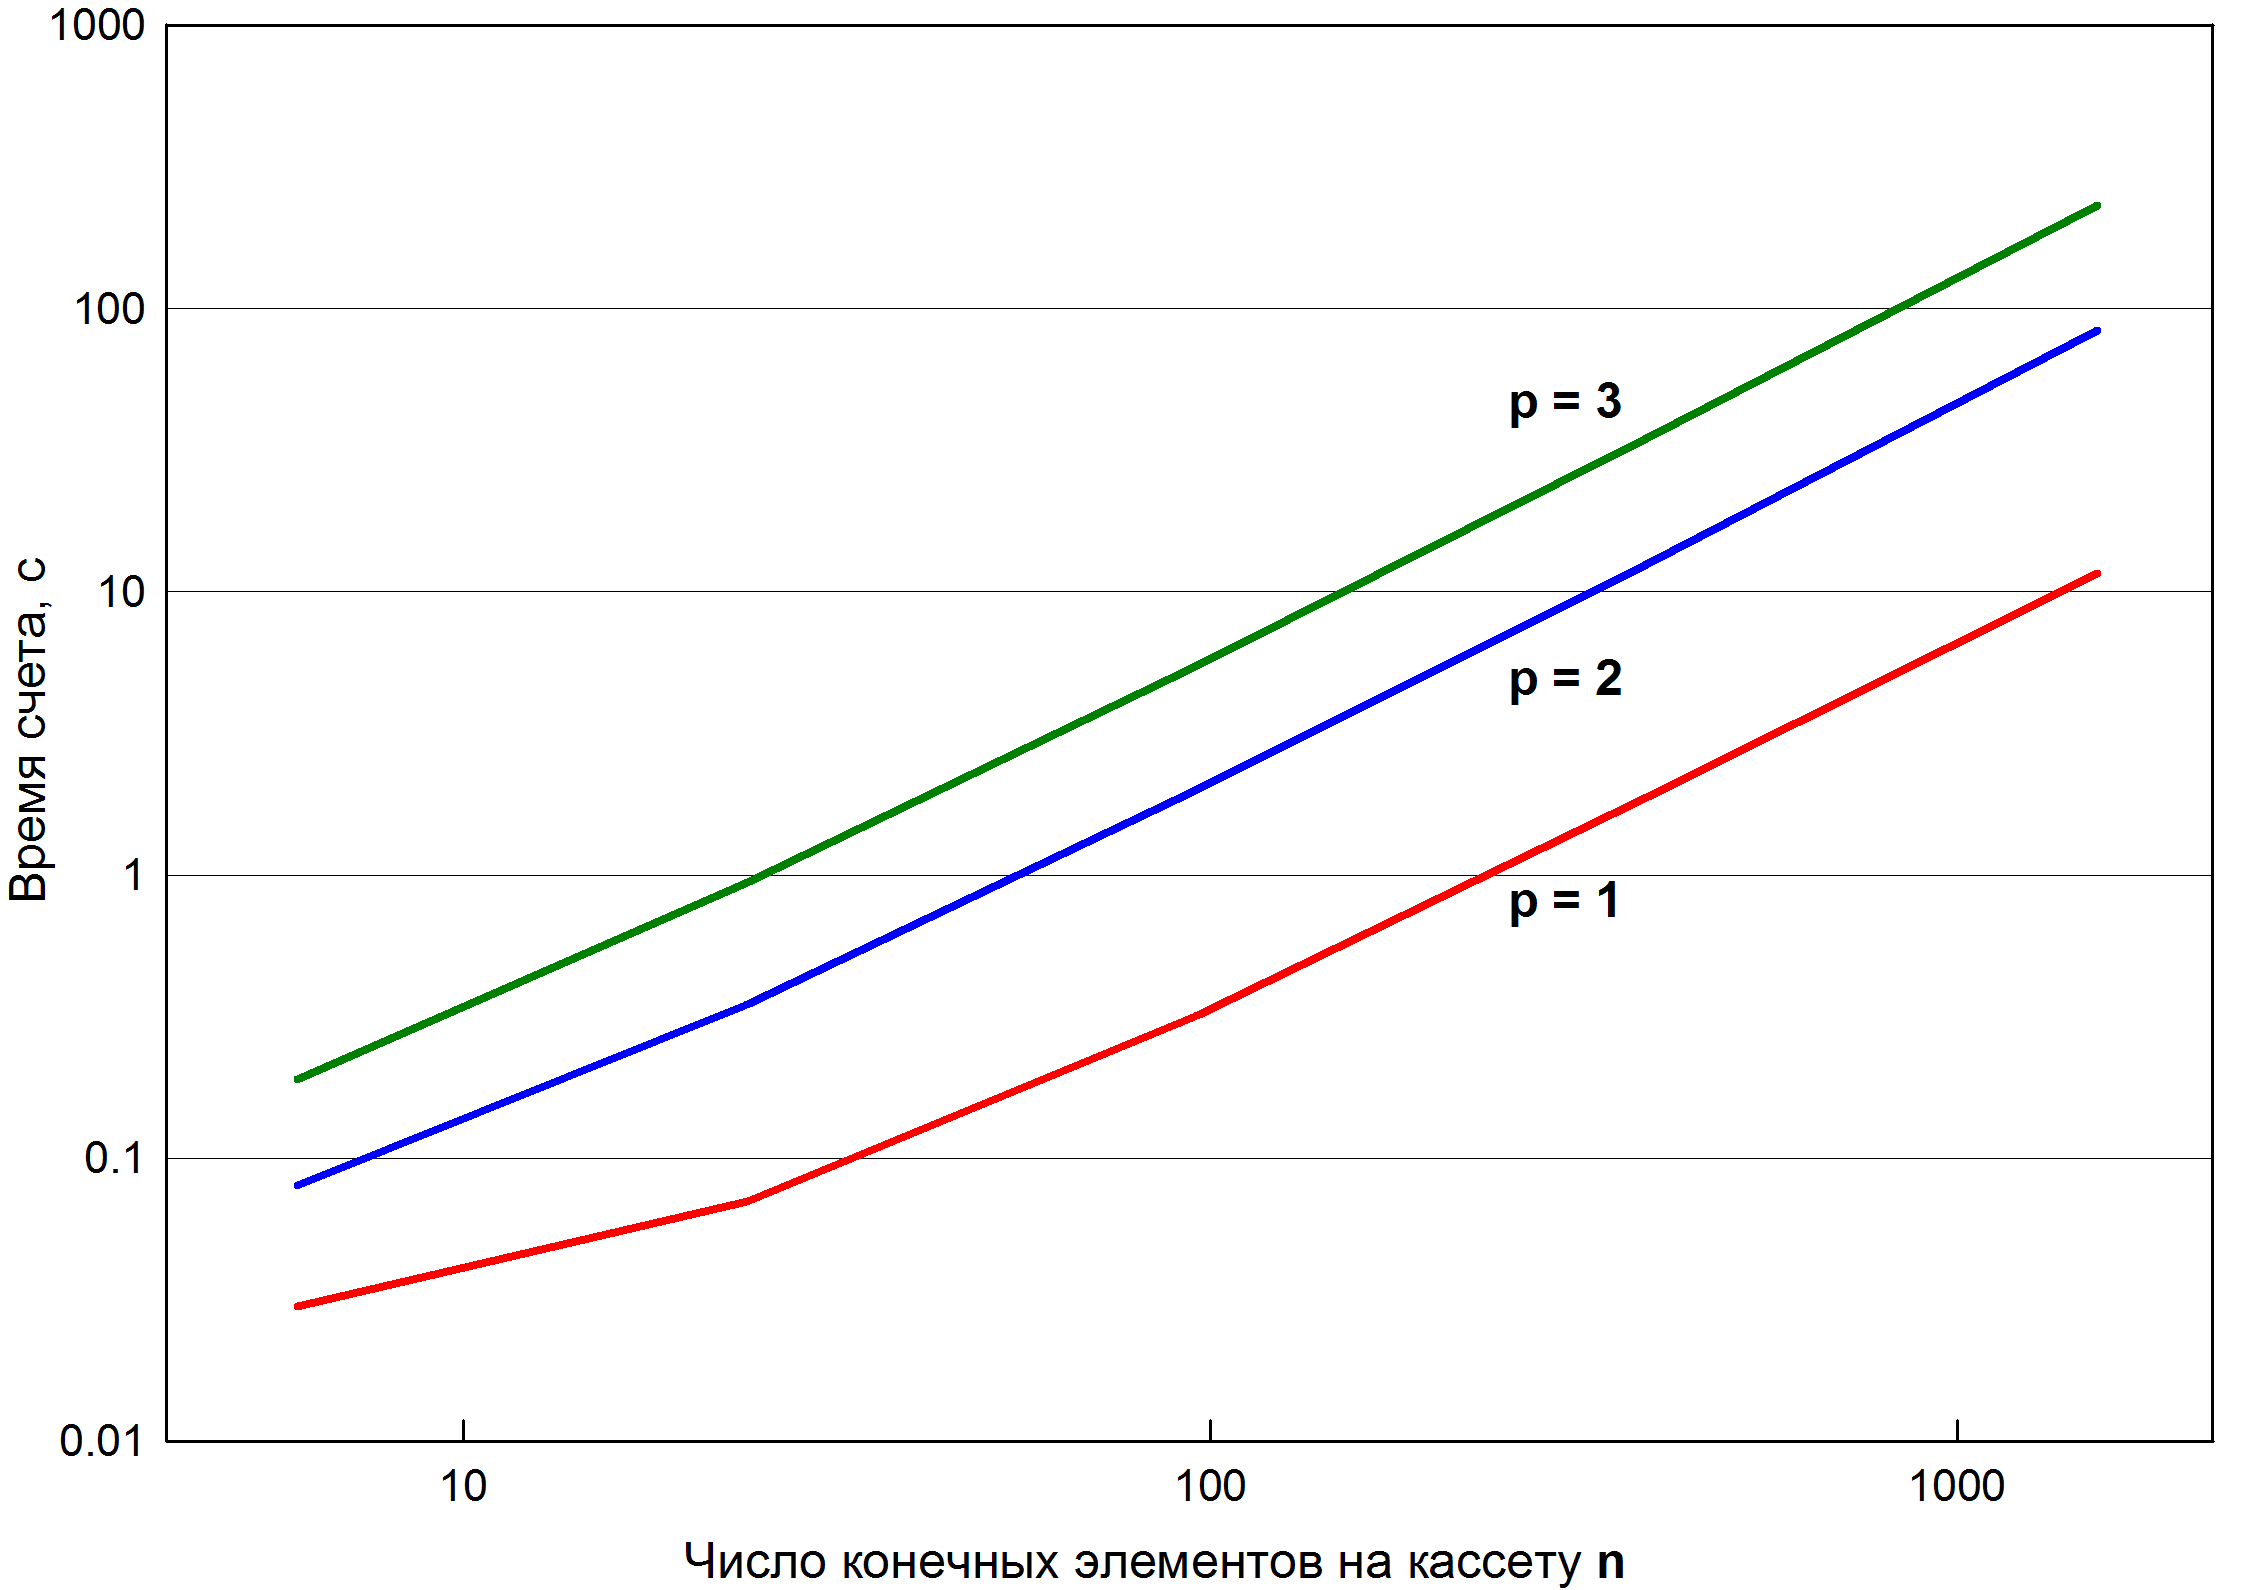
\includegraphics[width=0.9\linewidth]{Time.png}\\
	\caption{\label{image:canonsummary}Время счета задачи, t.}
	\label{ris:graph1}
\end{figure}
$\phantom{123}$
\\
Из рисунков 12-14, а также таблиц 2-5, 7 и 8 можно сделать следующие выводы: 
\begin{itemize}\itemsep1pt \parskip0pt \parsep0pt
\item наблюдается устойчивая сходимость решения тестовых задач при увеличении числа конечных элементов на кассету $n$ и порядка конечных элементов $p$;
\item с точки зрения экономичности расчета, увеличение порядка конечных элементов $p$ намного эффективнее увеличения числа конечных элементов на кассету $n$;
\item расчет с использованием конечных элементов первого порядка ($p = 1$) с малым числом конечных элементов на кассету ($n = 6$ или $24$) дает неудовлетворительные результаты; 
\item определены параметры «оптимального» варианта, удовлетворяющего выбранным критериям «приемлемости» результатов с точки зрения достижения достаточной для практических расчетов ВВЭР точности:
\begin{itemize}\itemsep1pt \parskip0pt \parsep0pt
\item $n = 6$; $p = 2$ для тестов IAEA-2D и модели ВВЭР-1000 без отражателя;
\item $n = 6$; $p = 3$ для тестов IAEA-2D с отражателем.
\end{itemize}
\end{itemize}
$\phantom{123}$
\\\\\\\\ \\\\\\\\ \\\\\\\\  \\\\\\\\ \\\\\\\\ 

\pagebreak
\section{Заключение}
\label{s-5}
\begin{enumerate} \itemsep1pt \parskip0pt \parsep0pt
\item Рассмотрено уравнение диффузии нейтронов в гексагональной геометрии, которое в операторном виде представляет спектральную задачу. Искались наименьшее собственное число и соответствующая ему собственная функция, которые характеризуют эффективный коэффициент размножения нейтронов и пространственное распределение плотности нейтронного потока соответсвенно. \item Разработан алгоритм решения спектральной задачи на основе метода конечных элементов. Написан программный код на основе разработанного алгоритма использующий вычислительную библиотеку FEniCS и библиотеку для решения спектральных задач SLEPc. 
\item Проведено тестирование разработанного программного кода на следующих двухмерных тестах, с различными граничными условиями:
\begin{itemize} \itemsep1pt \parskip0pt \parsep0pt
\item модифицированный тест IAEI-2D без отражателя;
\item модифицированный тест IAEI-2D с отражателем;
\item модель ВВЭР-1000 без отражателя.
\end{itemize} 
\item Исследовалась сходимость метода в зависимости от числа конечных элементов на кассету $n$ и порядка конечных элементов $p$. Разработанный алгоритм демонстрирует быструю сходимость и высокую точность при значениях $n = 6$ и $p = 2$ или $3$;
%\item Необходимо проанализировать влияние отражателя на сходимость метода. В качестве альтернативы увеличению порядка конечных элементов $p$ можно рассмотреть локальное сгущение расчетной сетки вблизи границы активной зоны с отражателем.
\end{enumerate}
$\phantom{123}$
\\\\\\\\\\\\\\\\
	\pagebreak
	
	\bibliographystyle{unsrt}
%	\bibliographystyle{utf8gost780s}
	\bibliography{article}


\end{document}
